\documentclass[12pt,oneside]{book}

% ─── Paquetes de Estética y Tipografía ─────────────────────────────────────
\usepackage[utf8]{inputenc}
\usepackage[T1]{fontenc}
\usepackage{lmodern}
\usepackage[spanish, es-tabla]{babel}
\usepackage{amsmath, amssymb, amsthm}
\usepackage{mathtools}
\usepackage{geometry}
\usepackage{setspace}
\usepackage{microtype}
\usepackage[colorlinks=true, linkcolor=blue, citecolor=blue, urlcolor=blue]{hyperref}
\usepackage[round, authoryear]{natbib}   % citas tipo (Autor, año)
\usepackage{booktabs}
\usepackage{longtable}
\usepackage{enumitem}
\usepackage{array}
\usepackage{titlesec}
\usepackage{fancyhdr}
\usepackage{graphicx}
\usepackage{multirow}
\usepackage{pgfplots}
\pgfplotsset{compat=1.18}

% ─── Configuración de Página ───────────────────────────────────────────────
\geometry{
    paper=a4paper,
    top=3cm,
    bottom=3cm,
    left=3.5cm,
    right=2.5cm
}
\onehalfspacing
\setlength{\emergencystretch}{2em}

% ─── Estilo de títulos de capítulos ───────────────────────────────────────
\titleformat{\chapter}[display]
  {\normalfont\huge\bfseries}{\chaptertitlename\ \thechapter}{20pt}{\Huge}
\titlespacing*{\chapter}{0pt}{-20pt}{40pt}

% ─── Teoremas y Operadores ─────────────────────────────────────────────────
\newtheorem{definition}{Definición}[chapter]
\newtheorem{remark}{Observación}[chapter]
\DeclareMathOperator{\E}{\mathbb{E}}
\DeclareMathOperator{\Prob}{\mathbb{P}}
\newcommand{\bps}{\,\text{bps}}

\graphicspath{{figuras/}}

\begin{document}

% ─── PORTADA INSTITUCIONAL ─────────────────────────────────────────────────
\begin{titlepage}
    \centering
    \vspace*{1cm}
    {\Large \textbf{PONTIFICIA UNIVERSIDAD JAVERIANA}} \\
    \vspace{0.5cm}
    {\large FACULTAD DE CIENCIAS} \\
    {\large DEPARTAMENTO DE MATEMÁTICAS} \\
    \vfill
    {\LARGE \textbf{Market Making con Aprendizaje Estadístico:}} \\
    \vspace{0.4cm}
    {\Large \textit{Un Enfoque Semiparamétrico para la Estimación Dinámica
    de Intensidades de Órdenes}} \\
    \vfill
    {\large \textbf{Santiago Rueda}} \\
    \vfill
    Trabajo de grado para optar al título de: \\
    \textbf{Científico de Datos} \\
    \vfill
    Tutor: \\
    \textbf{Vladimir Moreno} \\
    \vfill
    Bogotá D.C., Colombia \\
    2026
\end{titlepage}

% ─── ÍNDICES ───────────────────────────────────────────────────────────────
\frontmatter
\tableofcontents
\listoftables
\listoffigures

\mainmatter

\chapter*{Resumen}
\addcontentsline{toc}{chapter}{Resumen}
\markboth{Resumen}{Resumen}

Este trabajo evalúa si una mejor estimación de la llegada de órdenes agresivas mejora las decisiones de \textit{market making} en BTC/USDT de Binance Spot. Distingue dos resultados: la calidad de la predicción y el valor económico de las cotizaciones derivadas de ella. Se propone la intensidad semiparamétrica
$\lambda_i(t,\delta\mid X_t)=\exp\{g_i(X_t)+h_i(t)+m_i(X_t)f_i(\delta)\}$,
con 49 covariables causales, periodicidad horaria y una curva monótona de distancia modulada por estado. Predice alcance, no ejecución propia con prioridad en la cola.

La evaluación utiliza una captura propia del libro a 100~ms, con veinte niveles por lado, y 337 millones de transacciones entre el 29 de junio y el 26 de octubre de 2026. E3 tesis se compara con Avellaneda--Stoikov, Hawkes y un modelo lineal con las mismas covariables, reforzando las referencias. Se emplean cinco ventanas \textit{walk-forward} (34 días), un test de 17 días y una evaluación posterior de 36 días con modelos congelados. El test y parte del último periodo habían sido consultados con versiones anteriores; no son bloques completamente ciegos.

E3 mejora la puntuación predictiva frente a las referencias principales y obtiene AUC de 0,81 en el test y de aproximadamente 0,85 en el periodo posterior. El mejor Hawkes recupera el 74\,\% de su mejora sobre AS en el test y el modelo lineal, alrededor del 90\,\%. Frente a E3 sin covariables de barrido, la ventaja global en el lado ask no es significativa en los dos periodos finales. La calibración tras barridos mejora, pero no cumple el criterio fijado en el periodo posterior.

La mejora predictiva cambia las cotizaciones HJB con coeficientes congelados, pero no establece rentabilidad. Con cruce estricto, las políticas pierden aproximadamente entre 1,1 y 1,3~bps brutos por ejecución: el movimiento desfavorable alrededor de las ejecuciones supera el margen capturado. La FIFO aproximada produce resultados similares. Con ejecución optimista al toque, la HJB con E3 sí obtiene ganancias brutas pequeñas en el periodo posterior: $+0{,}15$~bps con E3 tesis y $+0{,}44$ con E3 base. Este escenario no estima la prioridad real y las ganancias no cubren las comisiones evaluadas de 7,5--10~bps. La contribución principal es predictiva; la evaluación económica delimita las condiciones bajo las cuales esa mejora no se tradujo en rentabilidad.

\medskip
\noindent\textbf{Palabras clave:} market making, intensidades, modelos semiparamétricos, selección adversa.

\chapter*{Abstract}
\addcontentsline{toc}{chapter}{Abstract}
\markboth{Abstract}{Abstract}

This thesis evaluates whether improved estimation of aggressive order arrivals improves market-making decisions in Binance Spot BTC/USDT. It distinguishes predictive quality from the economic value of the resulting quotes. The proposed semiparametric intensity is
$\lambda_i(t,\delta\mid X_t)=\exp\{g_i(X_t)+h_i(t)+m_i(X_t)f_i(\delta)\}$,
using 49 causal order-book and trade covariates, an hourly effect, a monotone distance curve and state-dependent modulation. Its target is the reach of hypothetical quotes, rather than fills of an agent's own orders with queue priority.

The evaluation uses a self-collected 100~ms, 20-level order book and 337 million trades from 29 June to 26 October 2026. The proposal is compared with Avellaneda--Stoikov, Hawkes and a linear model with the same covariates; applicable improvements are also given to the benchmarks. Five walk-forward windows cover 34 days, followed by a 17-day test and a later 36-day evaluation with frozen models. Earlier specifications had already been evaluated on the test and part of the later period, so these blocks are not fully blind.

The proposal improves predictive scores over the main benchmarks and achieves AUC values of 0.81 in the test and approximately 0.85 in the later period. The best Hawkes model recovers 74\,\% of its gain over AS in the test, and the linear model about 90\,\%. Its aggregate advantage over E3 without sweep covariates is not significant on the ask side in either final period. Calibration after sweeps improves, but fails the prescribed criterion in the later period.

Improved prediction changes HJB quotes under frozen coefficients, but does not establish profitability. Under strict-cross execution, the policies lose approximately 1.1--1.3~bps per fill before fees: adverse price movements around fills exceed the captured margin. An approximate FIFO queue produces similar results. Optimistic execution at the touch gives the HJB policy small gross profits in the later period: +0.15~bps with the thesis specification and +0.44 with baseline E3. This scenario does not estimate actual queue priority, and the gains do not cover the evaluated fees of 7.5--10~bps. The main contribution is predictive; the economic evaluation identifies the conditions under which that improvement failed to translate into profitability.

% ═══════════════════════════════════════════════════════════════════════════
\chapter{Introducción}
% ═══════════════════════════════════════════════════════════════════════════

El market making constituye uno de los problemas centrales de la microestructura de
mercados modernos. Un agente que actúa como market maker provee liquidez continua al
mercado publicando simultáneamente cotizaciones de compra y venta, buscando capturar
la diferencia entre ambas ---el spread--- a cambio de asumir el riesgo de
inventario y el riesgo de selección adversa \citep{GlostenMilgrom1985}.

Con el auge de los mercados electrónicos y el trading algorítmico, el diseño de
estrategias óptimas de market making ha adquirido una relevancia tanto académica como
práctica considerable. El modelo seminal de \citet{AvellanedaStoikov2008} estableció
el marco de referencia: formulando el problema como uno de control estocástico en
tiempo continuo, los autores derivan cotizaciones óptimas en función del inventario
acumulado y la volatilidad del activo. Sin embargo, este modelo descansa sobre una
especificación restrictiva: las ejecuciones se describen mediante procesos de Poisson
condicionales con forma exponencial en la distancia y parámetros fijos, sin depender
explícitamente de covariables contemporáneas del LOB ni de la historia reciente de
eventos.

La evidencia empírica muestra las limitaciones de esta especificación. Los datos de
alta frecuencia muestran que la dinámica de llegada de órdenes exhibe
\textit{clustering} temporal, dependencias entre eventos consecutivos y una fuerte
sensibilidad al estado observable del libro de órdenes, fenómenos que los procesos
de Poisson con parámetros fijos no pueden reproducir \citep{BacryHawkes2015}. Esta
brecha entre el modelo y la realidad puede producir intensidades mal calibradas
y afectar tanto la política de cotización como el control del riesgo de inventario.

Este trabajo propone cerrar esa brecha integrando herramientas de aprendizaje
estadístico dentro del marco de control estocástico, mediante un modelo
semiparamétrico que estima las intensidades de órdenes como funciones del estado
observable del mercado. El caso de estudio empírico se desarrolla sobre BTC/USDT
en Binance Spot, un mercado de criptoactivos que opera de manera continua y sobre el
cual se implementó una captura propia de datos históricos de alta frecuencia
directamente desde la infraestructura pública de mercado de Binance.


El trabajo responde dos preguntas que se mantienen separadas a lo largo del documento. La primera es predictiva: cuánto mejora la propuesta la estimación de la intensidad de llegada de órdenes agresivas a cada distancia del precio medio, frente a Avellaneda--Stoikov y a un Hawkes bivariado que reciben las mismas mejoras aplicables. La segunda es económica: qué valor produce esa mejora cuando se traduce en una política de cotización, bajo una regla de ejecución, unos costos y un inventario comunes. Una contribución predictiva puede coexistir con un resultado económico negativo, siempre que ambos se sustenten con el mismo rigor. Eso es lo que se encuentra aquí.

Las contribuciones son cuatro:
\begin{enumerate}[nosep]
\item una especificación semiparamétrica de la intensidad que incorpora el estado del libro, la periodicidad, una curva monótona de distancia modulada por el estado y covariables de barridos;
\item una comparación con referencias reforzadas, en la que E1 y E2 reciben los mismos hallazgos que E3, evaluada con \textit{walk-forward} y con especificaciones finales congeladas sobre un periodo de test;
\item la resolución numérica de la ecuación HJB con intensidades dependientes del estado y su evaluación económica con la misma regla de ejecución para todos los modelos;
\item una explicación cuantitativa de por qué la mejora predictiva no se traduce en rentabilidad en BTC/USDT, apoyada en la literatura reciente y en una comparación con tres motores de simulación limitada a configuraciones anteriores del entrenamiento.
\end{enumerate}

El Capítulo~\ref{chap:marco-teorico} presenta el marco teórico, el Capítulo~\ref{chap:metodologia} la metodología, el Capítulo~\ref{chap:datos} la captura y reconstrucción de los datos y el Capítulo~\ref{chap:resultados} los resultados, primero los predictivos y después los económicos. El Capítulo~\ref{chap:discusion} los interpreta frente a la literatura y declara las limitaciones, y el Capítulo~\ref{chap:conclusiones} concluye.

% ═══════════════════════════════════════════════════════════════════════════
\chapter{Problema a Trabajar}
% ═══════════════════════════════════════════════════════════════════════════

Sea $m_t$ el precio medio del activo y $X_t \in \mathbb{R}^d$ un vector de variables
de mercado observables en el instante $t$ (spread actual, desequilibrio del libro de
órdenes, volatilidad realizada y volumen en ventanas causales). Se denotan por
$\lambda_0^a(t\mid X_t)$ y $\lambda_0^b(t\mid X_t)$ las intensidades base de trades
agresores que pueden alcanzar, respectivamente, una cotización pasiva en el ask o en
el bid. La intensidad de fill a una distancia elegida $\delta$ combina esa intensidad
base con una función decreciente de la distancia y una regla conservadora de ejecución
reconstruida mediante replay del LOB.

El problema central de este trabajo se articula en cuatro preguntas de investigación:

\begin{enumerate}[label=\textbf{P\arabic*.}]
  \item \textquestiondown{}Cómo modelar $\lambda_0^a(t\mid X_t)$ y $\lambda_0^b(t\mid X_t)$ como
        funciones del estado del mercado $X_t$ y del tiempo $t$ usando un enfoque
        semiparamétrico que preserve la interpretabilidad del modelo de control
        estocástico?
  \item \textquestiondown{}Qué diferencias en PnL neto y control de inventario se obtienen frente a
        Avellaneda--Stoikov y frente a una política basada en intensidades Hawkes?
  \item \textquestiondown{}Cómo impacta la estimación data-driven de las intensidades en la política
        óptima de cotización derivada vía la ecuación HJB?
  \item \textquestiondown{}El desempeño del estimador de $g(X_t)$ se mantiene fuera de muestra ante
        cambios de régimen, costos, latencia y especificaciones de inventario?
\end{enumerate}


\chapter{Justificación}

La propuesta se justifica por la necesidad de representar el estado del mercado, por la disponibilidad de datos verificables y por su viabilidad computacional.

\paragraph{Fundamento teórico.} Una intensidad con parámetros fijos no representa la dependencia temporal del flujo de órdenes. \citet{BacryHawkes2015} revisan evidencia de endogeneidad y agrupamiento en aplicaciones financieras de procesos de Hawkes. \citet{ContKukanovStoikov2014} documentan la relación entre desequilibrio del flujo y cambios de precio de corto plazo en acciones. \citet{MorariuPatrichiPakkanen2022} muestran que la excitación del flujo depende de variables de estado, como spread y desequilibrio. Estos resultados motivan una intensidad que combine memoria, periodicidad y covariables observables, sin presuponer que una mejor predicción produzca rentabilidad.

\paragraph{Pertinencia empírica.} BTC/USDT en Binance Spot permite estudiar un mercado continuo con datos públicos de alta frecuencia. \citet{BarucciEtAl2022} documentan patrones intradía y la importancia de los mercados denominados en USDT en la formación de precios de criptoactivos; \citet{FabreToke2025} aplican estimación Hawkes no paramétrica a su microestructura. La captura propia permite reconstruir el libro, verificar secuencias y conservar las transacciones originales. La evaluación compara así modelos sobre una base común y auditable.

\paragraph{Viabilidad.} Los métodos de árboles son adecuados para comparar relaciones no lineales en datos tabulares de dimensión moderada \citep{GrinsztajnEtAl2022}. El trabajo contrasta gradient boosting con random forest y elige el estimador según desempeño temporal y costo de cómputo. La combinación de esa estimación con una curva de distancia interpretable permite integrar el pronóstico en el control de inventario y evaluar por separado su calidad estadística y su utilidad económica.

% ═══════════════════════════════════════════════════════════════════════════
\chapter{Objetivos}
% ═══════════════════════════════════════════════════════════════════════════

\section{Objetivo General}

Desarrollar un modelo de market making que integre control estocástico, métodos
semiparamétricos y machine learning para la estimación dinámica de intensidades de
órdenes, evaluando su desempeño empírico sobre datos de alta frecuencia de mercados
de criptoactivos.

\section{Objetivos Específicos}

\begin{enumerate}[label=\textbf{OE\arabic*.}]
  \item Analizar el modelo de \citet{AvellanedaStoikov2008} como caso base,
        identificando la forma exponencial en la distancia, los parámetros fijos y
        sus implicaciones sobre la política óptima de cotización.
  \item Proponer un modelo semiparamétrico para las intensidades de órdenes de la
        forma $\lambda_0(t) = \exp\bigl(g(X_t) + h(t)\bigr)$, especificando el vector
        de covariables $X_t$ y el componente temporal $h(t)$ a partir de propiedades
        documentadas de los datos de alta frecuencia.
  \item Implementar y comparar métodos de machine learning como Gradient Boosting
        y Random Forest para la estimación del componente no
        paramétrico $g(X_t)$, usando datos L2 históricos de BTC/USDT en Binance Spot.
  \item Derivar y resolver numéricamente la ecuación HJB bajo las intensidades
        semiparamétricas estimadas, obteniendo la política óptima de cotización
        data-driven.
  \item Evaluar el impacto del modelo propuesto frente a Avellaneda--Stoikov y a una
        política basada en Hawkes mediante las métricas de PnL neto, riesgo de
        inventario y robustez ante cambios de régimen de mercado.
\end{enumerate}


% ═══════════════════════════════════════════════════════════════════════════
\chapter{Marco teórico}
\label{chap:marco-teorico}
% ═══════════════════════════════════════════════════════════════════════════

Este capítulo reúne los conceptos necesarios para formular y comparar tres enfoques de creación de mercado: el modelo de Avellaneda--Stoikov, una especificación basada en procesos de Hawkes y el modelo semiparamétrico propuesto. El hilo conductor es la intensidad con que las órdenes agresivas alcanzan una cotización pasiva a cada distancia del precio medio. En los tres casos, el creador de mercado observa el estado del libro, decide las distancias de sus cotizaciones y administra el compromiso entre capturar el spread, mantener inventario y exponerse a selección adversa.

\section{Microestructura del libro y selección adversa}
\label{sec:seleccion-adversa}

En un mercado electrónico de órdenes límite, el \textit{limit order book} (LOB) organiza las intenciones de compra y venta por precio y prioridad temporal. En el instante $t$, el mejor precio comprador es $b_t$ y el mejor vendedor es $a_t$; de ellos se obtienen el precio medio y el spread:
\begin{equation}
 m_t=\frac{a_t+b_t}{2},
 \qquad
 s_t=a_t-b_t.
 \label{eq:mid-spread}
\end{equation}
Si $q^{b}_{i,t}$ y $q^{a}_{i,t}$ son las cantidades en el nivel $i$ de compra y venta, dos resúmenes del estado son el desequilibrio de profundidad y el precio medio ponderado por profundidad:
\begin{equation}
 I^{(K)}_t=
 \frac{\sum_{i=1}^{K}q^{b}_{i,t}-\sum_{i=1}^{K}q^{a}_{i,t}}
 {\sum_{i=1}^{K}q^{b}_{i,t}+\sum_{i=1}^{K}q^{a}_{i,t}},
 \qquad
 \mu_t=\frac{a_tq^{b}_{1,t}+b_tq^{a}_{1,t}}
 {q^{b}_{1,t}+q^{a}_{1,t}}.
 \label{eq:imbalance-microprice}
\end{equation}
El segundo indicador es el precio medio ponderado por profundidad (\textit{weighted mid-price}), denominado microprecio en las covariables de la implementación. Pondera cada mejor precio por la cantidad disponible en el lado opuesto. No es el estimador dinámico de microprecio de \citet{Stoikov2018}, definido mediante expectativas de precios medios futuros; aquí se usa el indicador lineal como covariable del estado, sin estimar ese modelo dinámico. El \textit{order flow imbalance} (OFI) resume además los cambios del mejor nivel y se relaciona con las variaciones contemporáneas del precio \citep{ContKukanovStoikov2014}. Spread, profundidad, desequilibrio, microprecio, OFI, volatilidad reciente y flujo de transacciones forman así un estado más informativo que el precio medio por sí solo.

El creador de mercado mantiene un inventario $q_t$, que aumenta cuando se ejecuta su compra y disminuye cuando se ejecuta su venta. El valor de una ejecución pasiva a un horizonte fijo se describe con su \textit{markout}: para una venta a precio $p$ en el instante $\tau$,
\begin{equation}
 \mathrm{MK}_H=\frac{p-m_{\tau+H}}{p}\times10^4~\text{bps},
 \label{eq:markout}
\end{equation}
con el signo opuesto para una compra. El \textit{markout} suma la distancia capturada respecto del precio medio y el movimiento posterior del precio. En el modelo de \citet{GlostenMilgrom1985}, el spread compensa al creador de mercado por negociar con agentes mejor informados \citep{OHara1995}. \citet{DeLise2024} estudia, en un modelo discreto y mediante simulación empírica de futuros, cómo las ejecuciones de órdenes límite pueden coincidir con movimientos adversos y producir una deriva condicional desfavorable. Esta relación motiva evaluar el precio alrededor de las ejecuciones, sin presuponer que todas tengan el mismo resultado. Cuando el spread es mínimo, el margen capturado es reducido y puede quedar superado por ese movimiento adverso. Esa relación entre ejecución y movimiento desfavorable es la \emph{selección adversa}. El markout es un diagnóstico local a horizonte fijo: caracteriza el valor de las ejecuciones, sin identificar por sí solo una causa, y no equivale al PnL completo de una estrategia que mantiene y compensa inventario a lo largo del tiempo \citep{Menkveld2013}.

\section{Avellaneda--Stoikov como referencia estructural}

\citet{AvellanedaStoikov2008}, extendiendo el enfoque clásico de control de inventario de \citet{HoStoll1981}, formulan la creación de mercado como un problema de control estocástico. El precio de referencia sigue $dm_t=\sigma\,dW_t$, el agente cotiza a distancias $\delta_t^b=m_t-p_t^b$ y $\delta_t^a=p_t^a-m_t$, y las ejecuciones llegan como procesos de conteo con intensidades
\begin{equation}
 \lambda^b(\delta)=A e^{-k\delta},
 \qquad
 \lambda^a(\delta)=A e^{-k\delta}.
 \label{eq:as-intensity}
\end{equation}
$A$ fija la escala de llegada y $k$ la sensibilidad a alejar la orden del mercado. Con utilidad exponencial y aversión al riesgo $\gamma$, una aproximación conocida da el precio de reserva y el spread óptimo:
\begin{equation}
 r_t=m_t-q_t\gamma\sigma^2(T-t),
 \qquad
 \psi_t=\gamma\sigma^2(T-t)+\frac{2}{\gamma}\log\!\left(1+\frac{\gamma}{k}\right).
 \label{eq:as-quotes}
\end{equation}
Si el inventario es positivo, el precio de reserva baja, lo que favorece vender. El modelo es interpretable, pero sus supuestos son restrictivos para alta frecuencia: $A$ y $k$ son fijos, las llegadas no tienen memoria ni dependen del estado del libro y el proceso de precios evoluciona de forma independiente de las ejecuciones pasivas \citep{AvellanedaStoikov2008,LalorSwishchuk2024}. En este trabajo funciona como línea base estructural: sus parámetros se estiman solo con el entrenamiento y su política se somete a la misma regla de ejecución que las demás.

\section{Procesos puntuales y modelo de Hawkes}
\label{sec:hawkes-multiescala}

En un proceso de Poisson la intensidad no depende de la historia, mientras que las transacciones aparecen en ráfagas. Los procesos de Hawkes introducen autoexcitación: cada evento eleva temporalmente la probabilidad de nuevos eventos \citep{Hawkes1971,BacryHawkes2015}. Para las compras agresivas ($+$, que alcanzan el ask) y las ventas ($-$, que alcanzan el bid), un Hawkes bivariado con $M$ escalas de memoria es
\begin{equation}
 \lambda_i(t)=\mu_i+\sum_{j\in\{+,-\}}\sum_{m=1}^{M}\alpha^{(m)}_{ij}\int_0^{t^-}\beta_m e^{-\beta_m(t-u)}\,dN_j(u),
 \qquad i\in\{+,-\}.
 \label{eq:hawkes-multi}
\end{equation}
$\mu_i$ es la intensidad basal, $\alpha^{(m)}_{ij}$ mide el efecto de un evento de tipo $j$ sobre el tipo $i$ y $\beta_m$ la velocidad de olvido. La estacionariedad exige que el radio espectral de la matriz de ramificación $\sum_m\alpha^{(m)}$ sea menor que uno. Con una sola escala, la estimación tiende a capturar las ráfagas de fragmentación de órdenes (milisegundos) y no la persistencia a escala de segundos; dos escalas permiten separar ambas memorias. Los parámetros se estiman con el algoritmo EM que trata como latente la estructura de ramificación \citep{VeenSchoenberg2008,Ozaki1979}. Estos modelos se han usado para transacciones, precios y libros de órdenes en mercados tradicionales y de criptoactivos \citep{Bowsher2007,LuAbergel2018,RambaldiEtAl2017,MorariuPatrichiPakkanen2022,CestariEtAl2023}.

Para compararlo con los demás modelos en la misma escala de tiempo, el Hawkes se evalúa con el número esperado de eventos en el intervalo siguiente, dada la historia:
\begin{equation}
 \Lambda_i(t)=\int_0^{\Delta}\E\bigl[\lambda_i(t+u)\mid\mathcal F_t\bigr]\,du .
 \label{eq:lambda-predictiva}
\end{equation}
Como la esperanza condicional de los estados de excitación satisface una ecuación diferencial lineal, \eqref{eq:lambda-predictiva} tiene forma cerrada mediante la exponencial matricial.

\section{Intensidad semiparamétrica propuesta}
\label{sec:curva-distancia}

Sea $X_t$ el vector de covariables causales del libro y del flujo, y $y_{t\delta}$ el número de eventos agresores del intervalo $[t,t+\Delta)$ que alcanzan $m_t(1\pm10^{-4}\delta)$, con $\delta$ en bps. Se utiliza una especificación Poisson de trabajo para la media condicional:
\begin{equation}
\begin{aligned}
 y_{t\delta}\mid X_t&\sim\operatorname{Poisson}\bigl(\Delta\,\lambda_i(t,\delta\mid X_t)\bigr),\\
 \lambda_i(t,\delta\mid X_t)&=\exp\bigl\{g_i(X_t)+h_i(t)+m_i(X_t)\,f_i(\delta)\bigr\}.
\end{aligned}
 \label{eq:fkx}
\end{equation}
\begin{itemize}[nosep]
\item $g_i$ es una función flexible del estado, estimada con \textit{gradient boosting} \citep{Friedman2001}; \textit{random forest} \citep{Breiman2001} sirve de alternativa. En datos tabulares ninguna familia domina siempre, por lo que la elección descansa en validación temporal \citep{GrinsztajnEtAl2022}.
\item $h_i(t)$ recoge la periodicidad horaria con variables conocidas fuera de muestra.
\item $f_i(\delta)$ es una curva monótona de distancia, con $f_i(\delta_1)=0$ y no creciente.
\item $m_i(X_t)=\exp(b_i^\top z_t)$ modula la pendiente de la curva según un vector corto de covariables estandarizadas: si $m_i>1$, la intensidad se concentra cerca del precio medio; si $m_i<1$, la curva se aplana.
\end{itemize}
El enlace exponencial garantiza positividad. La especificación del anteproyecto, $\exp\{g_i+h_i\}e^{-k_i\delta}$, es el caso $f_i(\delta)=-k_i\delta$ y $m_i\equiv1$; Avellaneda--Stoikov es además el caso $g_i+h_i$ constante. La forma exponencial impone una caída a tasa constante con la distancia; empíricamente, la caída es más rápida cerca del precio medio y más lenta en la cola, y eso motiva la curva libre $f_i$.

Como un evento que alcanza $\delta_2$ alcanza también toda $\delta_1<\delta_2$, los conteos están anidados y la función
\begin{equation}
 \ell=\sum_t\sum_\delta\bigl[y_{t\delta}\log\lambda(t,\delta)-\Delta\,\lambda(t,\delta)\bigr]
 \label{eq:ll-compuesta}
\end{equation}
es una verosimilitud compuesta. Con $m_i\equiv1$ y $g_i+h_i$ fijos, la condición de primer orden para cada $f_j$ da $f_j=\log N_j-\log\sum_t\Delta e^{g_i+h_i}$. El segundo término es común a todas las distancias; la normalización $f_i(\delta_1)=0$ lo traslada al nivel y deja la curva en forma cerrada:
\begin{equation}
 f_j=\log\frac{N_j}{N_1},\qquad N_j=\sum_t y_{tj},
 \label{eq:f-cerrada}
\end{equation}
monótona porque el anidamiento hace $N_j$ no creciente. Cuando $m_i$ varía, $f$ se parametriza como $f_j=-\sum_{l<j}e^{\theta_l}(\delta_{l+1}-\delta_l)$ y $(\theta,b)$ se estiman por máxima verosimilitud. Con $m_i$ variable, $f_i(\delta_1)=0$ deja de ser solo una normalización: como $m_i$ multiplica a $f_i$, fija el punto de giro de la curva. En $\delta_1$ la intensidad no depende de $m_i$, y $m_i$ escala la caída relativa a $\delta_1$; anclar la curva en otra distancia daría otro modelo, no una reparametrización. La escala entre $f_i$ y $m_i$ queda fijada porque $m_i=1$ en el estado medio ($z_t=0$). La estimación completa alterna los ajustes de $g_i$, $h_i$ y la curva (\textit{backfitting}), principio relacionado con la regresión semiparamétrica parcialmente lineal \citep{RobinsonSemiparametric1988,SancettaLOB2024}.

Las covariables usan solo información disponible antes de decidir la cotización, y la respuesta corresponde al intervalo posterior; así se evita el sesgo de anticipación. Que una variable mejore la predicción no implica que modificarla cause más ejecuciones: la interpretación es predictiva, no causal.

\section{Control óptimo con inventario y la ecuación HJB}
\label{sec:hjb-teoria}

La intensidad estimada se integra al problema de control mediante recompensas de ejecución y penalizaciones de inventario. De forma esquemática, la política maximiza
\begin{equation}
 \E\!\left[\mathrm{PnL}_T-\phi\int_0^T q_t^2\,dt-\eta q_T^2\right].
 \label{eq:objective}
\end{equation}
Se consideran un precio $dS_t=\sigma\,dW_t$, cotizaciones $S_t-\delta^b_t$ y $S_t+\delta^a_t$ con intensidades $\Lambda_i(\delta)=A_ie^{-k_i\delta}$ distintas por lado, inventario $|q|\le Q$ y utilidad $-\exp\{-\gamma(X_T+q_TS_T)\}$ \citep{GuentLehalle2013,Gueant2017,CarteaEtAl2015}. Con el ansatz $u=-\exp\{-\gamma(x+qS+\theta(t,q))\}$, la ecuación de Hamilton--Jacobi--Bellman se reduce a $2Q+1$ ecuaciones diferenciales:
\begin{equation}
0=\partial_t\theta-\tfrac12\gamma\sigma^2q^2+\mathbf 1_{q<Q}\,H_b\bigl(\theta(t,q)-\theta(t,q+1)\bigr)+\mathbf 1_{q>-Q}\,H_a\bigl(\theta(t,q)-\theta(t,q-1)\bigr),
\label{eq:hjb-theta}
\end{equation}
con Hamiltoniano y distancia óptima
\begin{equation}
H_i(p)=\frac{A_i}{k_i+\gamma}\Bigl(1+\frac{\gamma}{k_i}\Bigr)^{-k_i/\gamma}e^{-k_ip},\qquad
\delta_i^*=p+\frac1\gamma\ln\Bigl(1+\frac{\gamma}{k_i}\Bigr),
\label{eq:hjb-H}
\end{equation}
donde $p_b=\theta(q)-\theta(q+1)$ y $p_a=\theta(q)-\theta(q-1)$. Para una intensidad general $\Lambda_i(\delta)$ la reducción es la misma, con $H_i(p)=\sup_\delta\Lambda_i(\delta)\bigl(1-e^{-\gamma(\delta-p)}\bigr)/\gamma$, que ya no tiene forma cerrada y se calcula numéricamente. El término $-\tfrac12\gamma\sigma^2q^2$ tiene la misma forma que la penalización de \eqref{eq:objective} con $\phi=\tfrac12\gamma\sigma^2$, pero los dos objetivos no son equivalentes en general: con utilidad exponencial, el Hamiltoniano pondera la distancia por $(1-e^{-\gamma(\delta-p)})/\gamma$, mientras que con \eqref{eq:objective} lo hace por $\delta-p$; ambos coinciden solo cuando $\gamma\to0$ \citep{Gueant2017}. En este trabajo se usa la utilidad exponencial y el inventario final se valora al precio medio; esta condición terminal no representa una liquidación ejecutada en el libro. Para horizontes largos, $\theta(\tau,q)=c\tau+\theta_\infty(q)$ y la política estacionaria depende solo de $\sigma^2/A_a$, de $A_b/A_a$ y de $(k_a,k_b)$.

\citet{GuentLehalle2013} obtienen la aproximación cerrada (GLFT) para $\gamma$ pequeño:
\begin{equation}
\begin{aligned}
 \delta^{*}_{b}(q)&\approx\tfrac1\gamma\ln\bigl(1+\tfrac{\gamma}{k_b}\bigr)+\bigl(q+\tfrac12\bigr)\omega_b,\qquad
 \delta^{*}_{a}(q)\approx\tfrac1\gamma\ln\bigl(1+\tfrac{\gamma}{k_a}\bigr)-\bigl(q-\tfrac12\bigr)\omega_a,\\
 \omega_i&=\sqrt{\tfrac{\sigma^2\gamma}{2k_iA_i}\bigl(1+\tfrac{\gamma}{k_i}\bigr)^{1+k_i/\gamma}} .
\end{aligned}
 \label{eq:glft}
\end{equation}
Estas expresiones suponen que $\Lambda_i(\delta)$ es la intensidad de \emph{ejecución} de la propia orden. Los datos permiten estimar la intensidad de \emph{alcance} de una cotización hipotética, que es una cota superior de la de ejecución porque no considera la posición en la cola; en este trabajo se usa como aproximación, y la evaluación económica aplica una regla de ejecución más estricta (Sección~\ref{sec:eval-economica}). Dos consecuencias son centrales. En GLFT la distancia base depende de $k_i$ y no de $A_i$: un modelo que solo mejora el nivel de la intensidad apenas mueve las cotizaciones. En la solución numérica, en cambio, el cociente $A_b/A_a$ entra de forma no lineal en \eqref{eq:hjb-theta}, y la política se sesga hacia un lado incluso con inventario nulo. En el límite sin aversión ni inventario, el agente maximiza $\Lambda_i(\delta)\,\delta$ en cada instante (regla miope), cuyo óptimo exponencial es $\delta^*=1/k_i$.

Cuando las intensidades dependen del estado, el problema exacto incluiría $X_t$ como variable de estado. Aquí se usa la aproximación de coeficientes congelados: en cada decisión se aplica la política estacionaria con los coeficientes vigentes. En este trabajo, ``política óptima'' o ``política HJB'' designa esa política, óptima para el problema con coeficientes fijos; no es la óptima del problema que incluye la dinámica de $X_t$.

\section{Evaluación predictiva y valor económico}
\label{sec:evaluacion-pronosticos}

La función \eqref{eq:ll-compuesta} no se interpreta como la puntuación logarítmica de la distribución verdadera \citep{GneitingRaftery2007}: los conteos anidados la hacen compuesta y los datos tienen sobredispersión, así que ningún Poisson es la distribución verdadera. Su justificación es más débil y suficiente: en cada celda $(t,\delta)$, $y\log\lambda-\Delta\lambda$ es una función de puntuación estrictamente consistente para la media, cuyo valor esperado se maximiza solo cuando $\Delta\lambda=\E[y_{t\delta}\mid X_t]$, sea cual sea la distribución de $y_{t\delta}$ \citep{Gneiting2011}. La suma sobre celdas conserva la propiedad, de modo que la comparación ordena los modelos por su predicción del número esperado de eventos, no por la distribución completa. La comparación principal es, por tanto, la diferencia de \eqref{eq:ll-compuesta} por intervalo entre dos modelos, fuera de muestra, complementada con:
\begin{itemize}[nosep]
\item la discriminación, mediante el AUC del evento ``al menos un cruce a $\delta=2$~bps en el segundo'' \citep{Fawcett2006}; un predictor constante obtiene 0,5;
\item la calibración, mediante el cociente entre cruces observados y esperados (O/E);
\item la \emph{parte de la mejora}, $(\ell_m-\ell_{\text{AS}})/(\ell_{\text{E3}}-\ell_{\text{AS}})$, que indica qué fracción de la ganancia de la propuesta sobre Avellaneda--Stoikov recupera cada referencia.
\end{itemize}
Los intervalos de un mismo día están correlacionados, de modo que la incertidumbre se estima con un \textit{bootstrap} por días \citep{EfronTibshirani1993}. Para que la selección de especificaciones no contamine la evaluación, se combinan validación \textit{walk-forward}, protocolos con los criterios escritos antes de ver resultados y una evaluación final con modelos congelados.

La precisión estadística no determina el valor económico \citep{LeitchTanner1991}. \citet{AlbersEtAl2025} documentan, con órdenes reales en el perpetuo de Bitcoin de Binance, una relación negativa entre probabilidad de ejecución y retorno posterior, y estudian señales de reversión para afrontarla. No establecen una condición necesaria de rentabilidad; su evidencia orienta la interpretación de nuestro estudio de spot, sin sustituirlo. \citet{DeLise2024} muestra la deriva desfavorable condicionada a la ejecución en un modelo discreto y una simulación empírica de futuros. \citet{LalorSwishchuk2024} muestran que incorporar ejecuciones adversas y probabilidades de fill no adverso más realistas deteriora el desempeño de la estrategia de control que examinan. El resultado se limita a esa comparación y no valida nuestra cola aproximada. \citet{CarteaWang2020} incorporan señales de corto plazo para mitigar la selección adversa, con parte del valor procedente de órdenes de mercado. Una intensidad alta no implica por sí sola movimiento adverso: esa relación debe medirse. El valor económico depende de ejecución, movimiento del precio, inventario \citep{Menkveld2013} y costos o devoluciones por proveer liquidez. La evaluación empírica distingue estas dimensiones.

% ═══════════════════════════════════════════════════════════════════════════
\chapter{Metodología}
\label{chap:metodologia}
% ═══════════════════════════════════════════════════════════════════════════

El diseño es cuantitativo, longitudinal y comparativo sobre una capa canónica del libro de órdenes y las transacciones de BTC/USDT, cuya construcción se describe en el Capítulo~\ref{chap:datos}. Responde por separado dos preguntas: cuánto mejora la propuesta la predicción de la intensidad (P1) y qué valor económico produce en una política de cotización (P2--P3).

\section{Variable respuesta}
La respuesta se define sobre \emph{eventos agresores}: transacciones con el mismo instante y el mismo lado, que corresponden a una orden agresiva que barre uno o varios niveles, con su precio extremo. Para cada segundo $[t,t+1)$ y cada distancia $\delta\in\{0{,}5;1;2;3;5;7{,}5;10;15;20\}$~bps se cuentan los eventos compradores que alcanzan $m_t(1+10^{-4}\delta)$ (lado ask) y los vendedores que alcanzan $m_t(1-10^{-4}\delta)$ (lado bid). Un segundo es válido solo si el libro es observable en todas sus filas. Que el precio alcance una cotización hipotética no implica que una orden pasiva se ejecute: la respuesta mide la intensidad de \emph{alcance}, que no depende de la posición en la cola y se utiliza como proxy de la intensidad de ejecución.

\section{Partición y protocolo}
\label{sec:particion}
\begin{center}\small
\begin{tabular}{@{}llp{.46\textwidth}@{}}\toprule
Bloque & Fechas (2026) & Uso\\\midrule
Entrenamiento & 29 jun.--3 sep. (67 días) & Desarrollo, \textit{walk-forward} y ajuste de los modelos finales\\
Test & 4--20 sep. (17 días) & Evaluación de los modelos finales congelados, predictiva y económica\\
Simulación & 21 sep.--26 oct. (36 días) & Evaluación única de los mismos modelos y políticas, sin ningún reajuste\\\bottomrule
\end{tabular}
\end{center}

Dentro del entrenamiento se desarrolló la especificación de E3 (covariables, hiperparámetros, curva de distancia) y se reforzaron las referencias. Después, el orden fue fijo:
\begin{enumerate}[nosep]
\item \textit{walk-forward} con cinco ventanas semanales expansivas: se ajusta desde el 29 de junio hasta el 31 de julio, 7, 14, 21 y 28 de agosto, y se evalúa en los siete días siguientes (34 días fuera de muestra);
\item ajuste de los modelos finales con todo el entrenamiento, que se guardan sin cambios posteriores;
\item evaluación del test;
\item simulación, una sola vez, con los modelos y las políticas congelados.
\end{enumerate}
Cada paso tuvo un protocolo con sus criterios escritos antes de correr. Antes de abrir la simulación se comprobó que su código reproduce exactamente un día del test.

\paragraph{Versiones de los modelos.} Los resultados provienen de dos versiones del ajuste, que se identifican en cada tabla:
\begin{itemize}[nosep]
\item \textbf{ajuste original}: el \textit{walk-forward} y los modelos finales con los que se evaluó primero el test;
\item \textbf{ajuste corregido}: una revisión posterior encontró que el último paso de la curva de E3 no verificaba la convergencia y que su gradiente omitía el recorte de $m(X)$. Se corrigió y se reestimó solo ese paso (la curva, su modulación y un ajuste de nivel) para E3 tesis y E3-fkX, con $g$ y $h$ fijos y convergencia comprobada de ese paso, sin tocar las demás variantes. El test predictivo repetido con el ajuste corregido coincide con el original a tres decimales en todas las métricas.
\end{itemize}
El \textit{walk-forward} se conserva con el ajuste original; la evaluación económica usa el ajuste corregido. Ningún parámetro ni hiperparámetro se estimó con el periodo de test. El periodo se evaluó más de una vez: las versiones posteriores corrigieron defectos del código señalados en revisiones, no se eligieron por su desempeño en el test y no cambiaron las conclusiones. El test no es ciego en sentido estricto, porque la versión original de E3 se había evaluado en esas fechas (Apéndice~\ref{app:ciegos}); lo que confirma son las especificaciones finales, que nunca se evaluaron allí.

\section{Modelos comparados}
\label{sec:modelos}
Para que la comparación no favorezca a la propuesta, cada mejora aplicable a las referencias se les dio también: la curva de distancia, el nivel horario, un Hawkes de dos escalas, siete señales de barrido y tendencia, y un modelo lineal con las mismas covariables de E3. La Tabla~\ref{tab:modelos} resume las once variantes; todas comparten respuesta, distancias, segundos y datos, y se ajustan por lado.

\begin{table}[htbp]
\centering\small
\caption{Variantes comparadas. $\nu(\text{hora})$: nivel horario; $f(\delta)$: curva monótona \eqref{eq:f-cerrada}; S: siete señales (cinco de barrido, tendencia a 15~min y a 1~h); X49: las 49 covariables de E3 en un modelo lineal (GLM de Poisson).}
\label{tab:modelos}
\begin{tabular}{@{}lp{.60\textwidth}@{}}\toprule
Variante & $\log\lambda_i(t,\delta)$\\\midrule
AS base & $a_i-k_i\delta$\\
AS + h + f & $\nu_i(\text{hora})+f_i(\delta)$\\
AS + S & $\nu_i(\text{hora})+\beta_i^\top S_t+f_i(\delta)$\\
GLM lineal & $\nu_i(\text{hora})+\beta_i^\top X_t+f_i(\delta)$, 49 covariables\\
Hawkes 1 esc. + h + f / + S & $\log\Lambda_i(t)+\dots$, Hawkes de una escala \eqref{eq:lambda-predictiva}\\
Hawkes 2 esc. + h + f / + S & $\log\Lambda_i(t)+\dots$, Hawkes de dos escalas \eqref{eq:hawkes-multi}\\
E3 base & $g_i(X_t)+h_i(t)-k_i\delta$, 44 covariables\\
E3-fkX & $g_i(X_t)+h_i(t)+m_i(X_t)f_i(\delta)$, 44 covariables\\
\textbf{E3 tesis} & \eqref{eq:fkx} con 49 covariables (44 + 5 de barrido)\\\bottomrule
\end{tabular}
\end{table}

$g_i$ es un \textit{HistGradientBoosting} con pérdida Poisson (tasa de aprendizaje 0,05; 15 hojas; al menos 2\,000 observaciones por hoja; 300 iteraciones; regularización L2 de 1) \citep{PedregosaEtAl2011}, con tres ciclos de \textit{backfitting}. En cada ciclo: (i) con la curva y $h$ fijas, se ajusta $g$ por Poisson sobre el total de eventos del segundo, usando como desplazamiento la suma de la curva sobre las distancias; (ii) se reestima $h$ como nivel por hora; (iii) con $g+h$ fijos, se estiman la curva $f$ y los coeficientes $b$ de $m(X)$ por máxima verosimilitud (L-BFGS con gradiente analítico). La identificación se obtiene fijando $f(\delta_1)=0$ (que además fija el punto de giro de la modulación; Sección~\ref{sec:curva-distancia}), centrando $h$ sobre las 24 horas y absorbiendo el nivel común en una constante. El número de ciclos es fijo; se verificó que la verosimilitud de entrenamiento aumenta en cada ciclo, sin un criterio formal de convergencia. Los Hawkes se estiman con un tercio de los días de cada ventana, por costo computacional; sus capas de nivel, forma y señales usan todos los días. La lista de covariables está en el Apéndice~\ref{app:trazabilidad}.

\section{Evaluación predictiva}
Se compara la log-verosimilitud \eqref{eq:ll-compuesta} por segundo, el AUC a $\delta=2$~bps (promedio de los AUC diarios) y la calibración tras barridos (Sección~\ref{sec:evaluacion-pronosticos}), con intervalos \textit{bootstrap} por días (2\,000 réplicas). Los criterios del \textit{walk-forward} son que E3 tesis supere a cada referencia en las cinco ventanas y con intervalo de confianza positivo. Los del test son cuatro: superar a las referencias principales con intervalo positivo, ganar al menos 14 de 17 días al mejor Hawkes, un AUC de al menos 0,80 y un error de calibración tras barridos de a lo sumo 0,15.

\section{Evaluación económica}
\label{sec:eval-economica}
Todas las intensidades se evalúan en el test con el mismo simulador:
\begin{itemize}[nosep]
\item cada segundo y en cada lado se cotiza una orden de 0,01~BTC a la distancia que indica la política, redondeada al tick y siempre pasiva;
\item la orden se ejecuta solo si, dentro de ese segundo, un agresor negocia a un precio \emph{estrictamente} más allá del suyo (regla de cruce estricto). La regla no modela la cola: omite las ejecuciones al mismo precio de la orden, por lo que tiende a contar menos ejecuciones, pero no garantiza que el PnL resultante sea conservador; su sensibilidad a la cola se estudia en la Sección~\ref{sec:p2-origen};
\item la decisión usa el estado de la capa al inicio del segundo y la orden queda activa desde ese instante, sin latencia de envío; la sensibilidad a la latencia se estudió por separado en el entrenamiento (Sección~\ref{sec:p2-origen});
\item el inventario se limita a $|q|\le10$ y se valora al último precio medio del día.
\end{itemize}
Se evalúan tres políticas: la regla miope $\delta^*=\arg\max_\delta\lambda(\delta)\,\delta$; la política HJB numérica (Sección~\ref{sec:hjb-teoria}) con $\gamma=0{,}01$, elegido en la fase de desarrollo con la versión original de los modelos, y $Q=10$; y su aproximación GLFT. Para la HJB, la intensidad de cada modelo se usa con su curva de distancia interpolada entre los nueve nodos (Sección~\ref{sec:politica}); GLFT, cuya forma cerrada solo existe para intensidades exponenciales, usa en cada segundo un ajuste exponencial en $\delta\le5$~bps. La volatilidad es una media móvil exponencial causal, común a todos, con vida media de 60~s. Unidades: distancias y precios en bps del precio medio, tiempo en segundos, $A_i$ en eventos por segundo, $k_i$ en bps$^{-1}$, $\sigma$ en bps$/\sqrt{\text{s}}$, inventario $q$ en órdenes de 0,01~BTC y $\gamma$ en bps$^{-1}$ por orden.

Se reportan el PnL por ejecución y por día antes de comisiones, los días positivos, el número de ejecuciones, el inventario medio y el \textit{markout} a 10~s. El PnL de un día es el efectivo final más el inventario valorado al último precio medio, en USDT. El PnL por ejecución en bps es $10^4\times$ la suma del PnL de los días dividida por la suma del valor negociado (precio de cada ejecución por 0,01~BTC); su intervalo de confianza se obtiene remuestreando días.

% ═══════════════════════════════════════════════════════════════════════════
\chapter{Datos: captura, reconstrucción y capa canónica}
\label{chap:datos}
% ═══════════════════════════════════════════════════════════════════════════

Los datos de este trabajo no provienen de un proveedor comercial: se capturaron en vivo desde la infraestructura pública de Binance y se reconstruyó con ellos el libro de órdenes completo de BTC/USDT en Binance Spot. Este capítulo describe cómo se hizo y cómo se verificó.

\section{Captura en vivo}
Un servidor dedicado en Alemania se conectó de forma continua a dos flujos públicos de Binance Spot para BTC/USDT: el flujo de profundidad, que publica cada 100~ms los cambios del libro, y el flujo de transacciones, que publica cada operación con su precio, cantidad, lado agresor y hora del motor de negociación. Cada flujo se capturó dos veces en paralelo (captura primaria y de respaldo), de modo que un mensaje perdido por una conexión pudiera recuperarse de la otra. Los archivos se rotaron cada 12 horas y cada mensaje se guardó sin modificar, junto con su hora de recepción local. Periódicamente se descargaron instantáneas completas del libro, que sirven de punto de partida para la reconstrucción.

Las horas registradas permiten medir los retrasos. Binance publica cada transacción alrededor de 1~ms después de ejecutarla. La red añade una mediana de 127--131~ms hasta el servidor (percentiles 5 y 95 de unos 120 y 145~ms). Los mensajes de profundidad llegan en lotes regulares cada 100~ms, sin hora propia para cada cambio dentro del lote.

\section{Reconstrucción del libro}
El libro se reconstruyó siguiendo el procedimiento oficial de Binance para mantener un libro local \citep{BinanceSpotWebSocketDocs}:
\begin{enumerate}[nosep]
\item se parte de una instantánea completa del libro;
\item se aplican los mensajes de profundidad en orden, verificando que sus números de secuencia sean consecutivos;
\item las capturas primaria y de respaldo se combinan por número de secuencia, sin duplicar mensajes;
\item si falta un tramo de secuencia que ninguna captura cubre, el libro se marca como inválido hasta la siguiente instantánea, y ese intervalo nunca se interpola.
\end{enumerate}
Las transacciones se contrastaron con el archivo histórico oficial de Binance, que tiene la hora del motor con resolución de microsegundos; ese archivo se usó para verificar y completar transacciones, nunca para fabricar cambios del libro.

\section{Capa canónica}
A partir del libro reconstruido y de las transacciones se construyó una capa de estado cada 100~ms para el periodo del 29 de junio al 26 de octubre de 2026: 120 días, 864\,000 filas por día y 202 columnas. Cada fila contiene los veinte mejores niveles de cada lado, indicadores de validez y variables causales del libro, del flujo de transacciones y de la volatilidad, calculadas solo con información anterior a la fila. Las 337 millones de transacciones del periodo se conservan por separado, una por una. Toda la capa se construyó con el mismo código, y cada archivo queda registrado en un catálogo que permite verificar su integridad.

La Tabla~\ref{tab:volumen} resume el volumen de datos. El inventario del servidor al 19 de octubre registra 85~GB comprimidos capturados desde el 29 de junio (113 días): 64~GB de libros, 19~GB de transacciones y 2~GB del archivo oficial de Binance. Esa cifra incluye una captura paralela de Coinbase (BTC/USD), que se usó solo en la fase exploratoria. La parte de Binance BTC/USDT, con primaria y respaldo, suma unos 40~GB en esos 113 días. Coincide con lo medido en dos días completos conservados (27 y 28 de julio), que extrapolado a los 120 días da unos 42~GB comprimidos y 430~GB sin comprimir. Cada captura recibió unos 862\,800 mensajes de profundidad al día, de 864\,000 posibles (99,9\,\%), y las dos capturas difieren en pocos cientos de mensajes por día. Unos 880 millones de mensajes crudos se convierten así en una capa de 38~GB lista para modelar.

\begin{table}[htbp]
\centering\small\setlength{\tabcolsep}{4pt}
\caption{Volumen de los datos crudos y de la capa canónica.}
\label{tab:volumen}
\begin{tabular}{@{}lrrr@{}}
\toprule
 & Mensajes o filas & Comprimido & Sin comprimir\\\midrule
Servidor, todo (medido, 113 días) & --- & 85~GB & ---\\
Binance, primaria (120 días) & $\approx$440 millones & $\approx$21~GB & $\approx$214~GB\\
Binance, ambas capturas (120 días) & $\approx$880 millones & $\approx$42~GB & $\approx$430~GB\\
Canónica: libro (202 columnas) & 104 millones de filas & 35~GB & ---\\
Canónica: transacciones & 337 millones & 3~GB & ---\\
\bottomrule
\end{tabular}
\end{table}

\section{Verificaciones}
La Tabla~\ref{tab:auditoria} resume las verificaciones.

\begin{table}[htbp]
\centering\small
\caption{Verificaciones de la reconstrucción y de la capa canónica.}
\label{tab:auditoria}
\begin{tabular}{@{}p{.70\textwidth}r@{}}
\toprule Verificación & Resultado\\\midrule
Tramos entre instantáneas cuyo libro reconstruido coincide exactamente con la instantánea siguiente (100 niveles por lado) & 103 de 116\\
Instantáneas posteriores con fila correspondiente que coinciden exactamente en 20 niveles & 18 de 18\\
Conflictos de precio o cantidad entre transacciones capturadas y el archivo oficial & 0\\
Mejores precios distintos frente a una reconstrucción independiente (22,9 millones de filas comparadas) & 2 por lado\\
Libros cruzados, niveles desordenados o cantidades no positivas & 0\\
Fracción mínima de filas válidas en un día & 99,95\,\%\\
Tiempo con spread de un tick (0,01~USDT), entrenamiento & 99,96\,\%\\
\bottomrule
\end{tabular}
\end{table}

Los 13 tramos que no coinciden contienen huecos de secuencia; quedaron marcados como inválidos y no se usaron. Las pequeñas diferencias de profundidad frente a la reconstrucción independiente (0,01--0,04\,\% de las filas) se concentran en niveles alejados del mejor precio.

\section{Causalidad y alineación de relojes}
\label{sec:datos-resultados}

Las covariables deben usar solo información anterior a cada decisión. Para comprobar que la capa no contiene información del intervalo que se quiere predecir se midió, para cada transacción agresiva que barre varios niveles, la fracción de casos en que el libro vigente $s$ milisegundos después del evento ya refleja el barrido. Si hubiera fuga, el barrido aparecería en $s\le0$. La fracción se mantiene en el nivel de fondo (cerca de 1\,\%) hasta $s=80$~ms, sube desde $s\approx90$~ms y se completa hacia $s\approx200$~ms (Figura~\ref{fig:reloj}).

\begin{figure}[htbp]
\centering
\begin{tikzpicture}
\begin{axis}[width=.9\textwidth,height=5.6cm,xlabel={Desfase $s$ respecto al evento (ms)},ylabel={Barridos ya reflejados (\%)},
 xmin=-200,xmax=300,ymin=0,ymax=100,ymajorgrids=true,grid style={gray!20},mark size=1.2pt]
\addplot[blue!70!black,mark=*] coordinates {(-200,2.70) (-180,2.55) (-160,2.36) (-140,2.20) (-120,2.06) (-100,1.90) (-80,1.73) (-60,1.56) (-40,1.39) (-20,1.25) (0,1.10) (20,0.95) (40,0.78) (60,0.63) (80,0.46) (100,11.48) (120,30.26) (140,49.13) (160,68.08) (180,85.20) (200,93.08) (220,93.53) (240,93.68) (260,93.71) (280,93.73) (300,93.69)};
\draw[dashed,gray] (axis cs:0,0) -- (axis cs:0,100);
\end{axis}
\end{tikzpicture}
\caption{Fracción de barridos multinivel ya reflejados en el libro $s$ milisegundos después del evento, 29 de junio de 2026 (155\,676 barridos). Otros días muestran el mismo patrón.}
\label{fig:reloj}
\end{figure}

No hay fuga detectable: el libro va unos 90~ms detrás del reloj de las transacciones, por la publicación en lotes de 100~ms. Un participante real vería además el estado con el retraso de red. Por eso se verificó, con la versión original de E3, que un retraso adicional de 200~ms en las covariables conserva entre el 81 y el 90\,\% de su ventaja predictiva.

% ═══════════════════════════════════════════════════════════════════════════
\chapter{Resultados}
\label{chap:resultados}
% ═══════════════════════════════════════════════════════════════════════════

El capítulo sigue el orden de las preguntas. La Sección~\ref{sec:especificacion-final} resume cómo se llegó a la especificación final de E3; es la única parte exploratoria del capítulo. Las Secciones~\ref{sec:walkforward} a~\ref{sec:rebote} responden P1 (mejora predictiva), la Sección~\ref{sec:politica} responde P3 (efecto sobre la política), las Secciones~\ref{sec:p2} y~\ref{sec:p2-origen} responden P2 (valor económico), y la Sección~\ref{sec:simulacion} repite ambas evaluaciones en un periodo posterior. Las diferencias de log-verosimilitud se expresan por segundo, sumando las nueve distancias; un valor positivo favorece a E3 tesis.

\section{Especificación final de E3}
\label{sec:especificacion-final}

La especificación se desarrolló dentro del entrenamiento, comparando siempre fuera de muestra por días. Cuatro resultados la definieron.

\paragraph{El estado del mercado explica la mayor parte de la intensidad.} La versión del anteproyecto, $\exp\{g(X)+h(t)\}e^{-k\delta}$ con 44 covariables, redujo a la mitad la log-verosimilitud negativa de Avellaneda--Stoikov en la fase de desarrollo y alcanzó un AUC de 0,84, frente a 0,50 de AS y 0,64--0,65 del Hawkes de una escala. En ablaciones por grupos, el flujo reciente de transacciones fue el más informativo, seguido del libro y de la volatilidad; el OFI resultó casi redundante. El componente horario mejora el lado ask pero no el bid, y se usa solo en el ask. Evaluada después sin reajustar, esa versión superó a AS todos los días de una validación y de dos tests ciegos, aunque uno de los tres veredictos preregistrados no se cumplió (Apéndice~\ref{app:ciegos}).

\paragraph{Gradient boosting frente a random forest (OE3).} Con la misma información, ambos estimadores de $g$ llegan a la misma conclusión: la log-verosimilitud difiere en menos del 1,2\,\% y el AUC en una milésima, en desarrollo y en validación. \textit{Random forest} cuesta entre 4 y 35 veces más tiempo de cómputo, por lo que \textit{gradient boosting} es el estimador principal.

\paragraph{La forma exponencial en la distancia estaba mal calibrada.} A 2~bps, la versión original predecía entre 1,6 y 1,9 veces los cruces observados. Reemplazar $-k\delta$ por la curva monótona \eqref{eq:f-cerrada} reduce el mayor desvío de $\log(O/E)$ entre distancias de 5,6 a 0,4 en el ask y de 8,1 a 2,3 en el bid, con una mejora de $+0{,}031$ y $+0{,}032$ por segundo en todos los días, sin cambio en el AUC. Modular la curva por el estado, $m(X)f(\delta)$, añade $+0{,}011$ a $+0{,}016$. La curva final cae a $f(2)=-1{,}64$ y $f(20)=-8{,}65$ en el ask ($-1{,}68$ y $-10{,}31$ en el bid): más rápido cerca del precio medio y más lento en la cola.

\paragraph{Faltaban covariables de barrido.} Tras un barrido comprador, el cociente estimado $\lambda_a/\lambda_b$ a 2~bps pasa de 1,3 a 5,6, de modo que E3 capta el impulso del barrido. Pero subestimaba el rebote del lado contrario: tras barridos vendedores llegaban cerca de un 60\,\% más compradores de los esperados. Cinco covariables causales (recorrido firmado, volumen y tiempo desde el último barrido; spread máximo y variación del precio medio en el último segundo) reducen esa brecha de 0,454 a 0,091.

La especificación final, \textbf{E3 tesis}, es \eqref{eq:fkx} con 49 covariables, $h$ horaria en el ask, curva $f$ monótona y $m(X)=\exp(b^\top z)$ con cuatro covariables. Sus coeficientes de modulación son pequeños ($|b_j|\le0{,}10$).


\section{P1: comparación con referencias reforzadas}
\label{sec:walkforward}

Las referencias reciben las mismas mejoras aplicables que E3 (Tabla~\ref{tab:modelos}). El Hawkes de dos escalas ajustado con todo el entrenamiento elige memorias de 1~s y 3,3~ms ($\beta=1$ y $300$~s$^{-1}$) con radio espectral 0,74; el de una escala elige solo la escala rápida.

La Tabla~\ref{tab:wf} y la Figura~\ref{fig:wf-parte} resumen los 34 días fuera de muestra del \textit{walk-forward}. La ventana 1 reproduce exactamente los resultados obtenidos antes con el mismo ajuste (diferencia relativa nula), lo que verifica el código.

\begin{table}[htbp]
\centering\footnotesize
\caption{\textit{Walk-forward} (cinco ventanas semanales, 34 días fuera de muestra; ajuste original). Parte de la mejora de E3 tesis sobre AS base que recupera cada modelo, ventaja de E3 tesis por intervalo [IC95 por días] y AUC a $\delta=2$~bps.}
\label{tab:wf}
\resizebox{\textwidth}{!}{%
\begin{tabular}{@{}lrrccrr@{}}\toprule
& \multicolumn{2}{c}{Parte de la mejora} & \multicolumn{2}{c}{E3 tesis $-$ modelo} & \multicolumn{2}{c}{AUC}\\
\cmidrule(lr){2-3}\cmidrule(lr){4-5}\cmidrule(l){6-7}
Modelo & ask & bid & ask & bid & ask & bid\\\midrule
\textbf{E3 tesis} & 100\,\% & 100\,\% & -- & -- & 0,834 & 0,825\\
E3-fkX (44 cov.) & 98,6\,\% & 99,5\,\% & $+0{,}024$ [0,005; 0,050] & $+0{,}008$ [0,002; 0,015] & 0,833 & 0,824\\
E3 base & 92,7\,\% & 93,5\,\% & $+0{,}127$ [0,058; 0,225] & $+0{,}110$ [0,045; 0,213] & 0,834 & 0,824\\
GLM lineal (49 cov.) & 90,9\,\% & 90,1\,\% & $+0{,}158$ [0,111; 0,223] & $+0{,}166$ [0,102; 0,254] & 0,821 & 0,814\\
Hawkes 2 esc. + S & 79,1\,\% & 75,8\,\% & $+0{,}365$ [0,275; 0,470] & $+0{,}408$ [0,286; 0,554] & 0,780 & 0,772\\
Hawkes 2 esc. + h + f & 61,7\,\% & 60,9\,\% & $+0{,}668$ [0,442; 0,962] & $+0{,}659$ [0,424; 0,959] & 0,757 & 0,752\\
Hawkes 1 esc. + S & 52,4\,\% & 49,0\,\% & $+0{,}830$ [0,593; 1,114] & $+0{,}860$ [0,565; 1,206] & 0,731 & 0,725\\
AS + S & 50,8\,\% & 47,0\,\% & $+0{,}857$ [0,609; 1,152] & $+0{,}893$ [0,582; 1,261] & 0,728 & 0,721\\
Hawkes 1 esc. + h + f & 9,2\,\% & 9,1\,\% & $+1{,}582$ [0,995; 2,303] & $+1{,}530$ [0,941; 2,240] & 0,628 & 0,626\\
AS + h + f & 7,4\,\% & 6,9\,\% & $+1{,}614$ [1,012; 2,352] & $+1{,}567$ [0,961; 2,294] & 0,616 & 0,612\\
AS base & 0\,\% & 0\,\% & $+1{,}743$ [1,122; 2,483] & $+1{,}684$ [1,061; 2,440] & 0,500 & 0,500\\\bottomrule
\end{tabular}}
\end{table}

\begin{figure}[htbp]
\centering
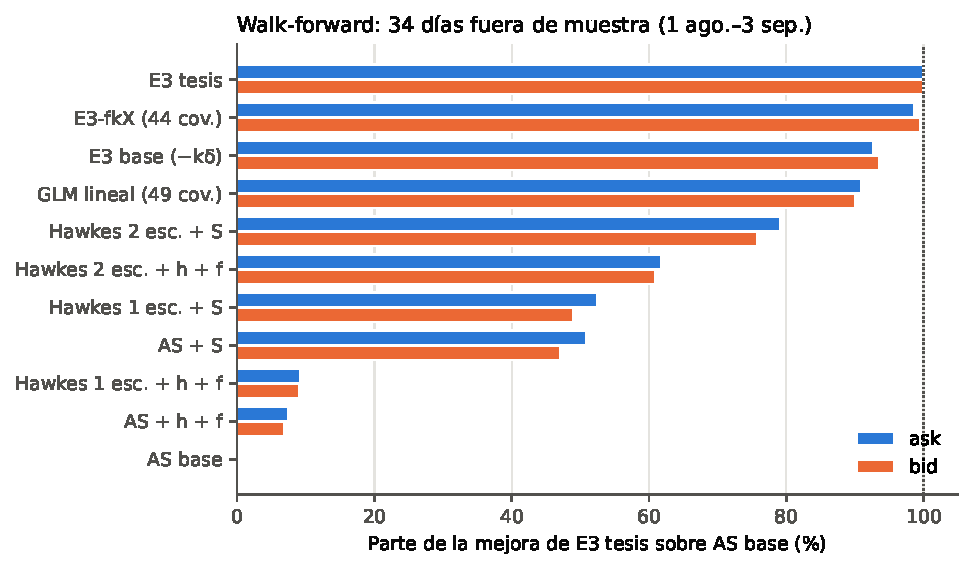
\includegraphics[width=.86\textwidth]{F1_parte_mejora_wf.pdf}
\caption{Parte de la mejora de E3 tesis sobre AS base que recupera cada modelo en el \textit{walk-forward}.}
\label{fig:wf-parte}
\end{figure}

Se cumplen los dos criterios principales del protocolo. \emph{Estabilidad}: E3 tesis supera a cada uno de los diez modelos en las cinco ventanas y en ambos lados (Figura~\ref{fig:wf-ventanas}). \emph{Diferencia global}: el intervalo de confianza de la ventaja es positivo frente a todos; frente a E3-fkX gana 25 y 23 de 34 días, y frente a los demás, 33 o 34 de 34. La ventaja crece en las semanas agitadas (15--28 de agosto), en las que una intensidad constante falla más.

\begin{figure}[htbp]
\centering
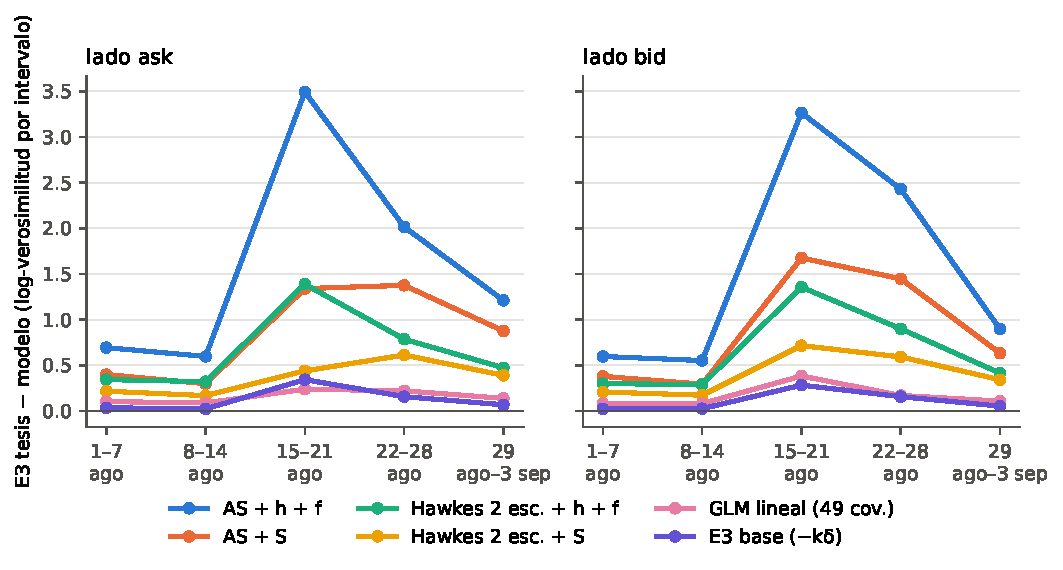
\includegraphics[width=.95\textwidth]{F2_ventaja_por_ventana.pdf}
\caption{Ventaja de E3 tesis sobre seis referencias en cada ventana del \textit{walk-forward}. Todas las curvas quedan por encima de cero.}
\label{fig:wf-ventanas}
\end{figure}

El diagnóstico de sobreajuste compara la ventaja de E3 sobre el GLM lineal en la semana siguiente con la de la última semana ajustada. El cociente está por debajo de 0,5 en dos de cinco ventanas (V4 y V5), en las que la semana ajustada incluye el periodo agitado del 15 al 28 de agosto y la ventaja dentro de muestra se infla; el umbral del protocolo (tres ventanas) no se alcanza. En la ventana 3 el cociente supera 2, porque la semana evaluada es la agitada.

Tres lecturas se desprenden de la Tabla~\ref{tab:wf}. Primera, el estado del libro explica la mayor parte de la mejora: el GLM lineal con las mismas covariables recupera el 90--91\,\%. La no linealidad de $g$ aporta el resto, mejora la discriminación (AUC 0,834 frente a 0,821) y, entre los modelos evaluados, es la que mejor corrige el rebote (Sección~\ref{sec:rebote}). Segunda, la memoria importa, pero con la escala correcta: el Hawkes de dos escalas recupera el 61--62\,\% frente al 9\,\% del de una escala. Tercera, las variables de barrido aportan poco a la verosimilitud global (E3-fkX recupera el 98,6--99,5\,\%), porque los barridos son eventos raros; su valor está en la calibración tras esos eventos.


\section{P1: test final}
\label{sec:test}

Con los once modelos ajustados en todo el entrenamiento y congelados antes de leer el test, se evaluaron una sola vez en el test del 4 al 20 de septiembre, un periodo ya consultado con la versión original de E3. Se cumplen los cuatro criterios preregistrados (Tabla~\ref{tab:test}):
\begin{itemize}[nosep]
\item \textbf{jerarquía}: E3 tesis supera a AS + h + f, AS + S, GLM lineal, Hawkes 2 escalas + h + f y Hawkes 2 escalas + S con IC95 positivo en ambos lados;
\item \textbf{consistencia}: gana 17 de 17 días al Hawkes de dos escalas con señales en ambos lados;
\item \textbf{discriminación}: AUC de 0,813 en ambos lados, por encima de 0,80;
\item \textbf{rebote}: brecha de $+0{,}116$ tras barridos vendedores y $-0{,}139$ tras compradores, dentro de $\pm0{,}15$.
\end{itemize}

\begin{table}[htbp]
\centering\footnotesize
\caption{Test final (4--20 sep., 17 días; modelos congelados con el ajuste corregido, idéntico al original a tres decimales). Parte de la mejora sobre AS base, ventaja de E3 tesis por intervalo [IC95 por días] y días en que gana E3 tesis (ask / bid).}
\label{tab:test}
\resizebox{\textwidth}{!}{%
\begin{tabular}{@{}lrrccc@{}}\toprule
& \multicolumn{2}{c}{Parte de la mejora} & \multicolumn{2}{c}{E3 tesis $-$ modelo} & \\
\cmidrule(lr){2-3}\cmidrule(lr){4-5}
Modelo & ask & bid & ask & bid & Días\\\midrule
E3-fkX (44 cov.) & 99,8\,\% & 98,9\,\% & $+0{,}002$ [$-0{,}004$; 0,008] & $+0{,}015$ [0,003; 0,029] & 10 / 13\\
E3 base & 96,0\,\% & 93,5\,\% & $+0{,}053$ [0,034; 0,073] & $+0{,}087$ [0,047; 0,134] & 16 / 17\\
GLM lineal (49 cov.) & 91,6\,\% & 89,6\,\% & $+0{,}110$ [0,077; 0,145] & $+0{,}140$ [0,089; 0,193] & 16 / 16\\
Hawkes 2 esc. + S & 73,8\,\% & 73,7\,\% & $+0{,}345$ [0,251; 0,454] & $+0{,}353$ [0,263; 0,457] & 17 / 17\\
Hawkes 2 esc. + h + f & 60,3\,\% & 62,3\,\% & $+0{,}523$ [0,377; 0,692] & $+0{,}505$ [0,355; 0,681] & 17 / 17\\
Hawkes 1 esc. + S & 45,1\,\% & 44,6\,\% & $+0{,}723$ [0,494; 0,985] & $+0{,}742$ [0,510; 1,007] & 17 / 17\\
AS + S & 43,6\,\% & 43,0\,\% & $+0{,}742$ [0,508; 1,010] & $+0{,}764$ [0,526; 1,036] & 17 / 17\\
Hawkes 1 esc. + h + f & 11,1\,\% & 12,3\,\% & $+1{,}170$ [0,775; 1,644] & $+1{,}175$ [0,743; 1,678] & 17 / 17\\
AS + h + f & 9,5\,\% & 10,4\,\% & $+1{,}191$ [0,788; 1,671] & $+1{,}200$ [0,759; 1,714] & 17 / 17\\
AS base & 0\,\% & 0\,\% & $+1{,}316$ [0,880; 1,810] & $+1{,}340$ [0,835; 1,953] & 17 / 17\\\bottomrule
\end{tabular}}
\end{table}

El orden de los modelos es el mismo que en el \textit{walk-forward} (Figura~\ref{fig:test-parte}) y el AUC baja de 0,83 a 0,81, una degradación moderada en datos nuevos. Frente a E3-fkX, la ventaja en el lado ask no es significativa: las variables de barrido no mejoran la predicción global en ese lado, aunque sí la calibración del rebote. Los AUC de las referencias en el test son 0,80 (GLM), 0,76--0,77 (Hawkes 2 escalas + S), 0,74--0,75 (Hawkes 2 escalas + h + f), 0,71--0,72 (AS + S), 0,61--0,63 (AS y Hawkes 1 escala con h y f) y 0,50 (AS base).

\begin{figure}[htbp]
\centering
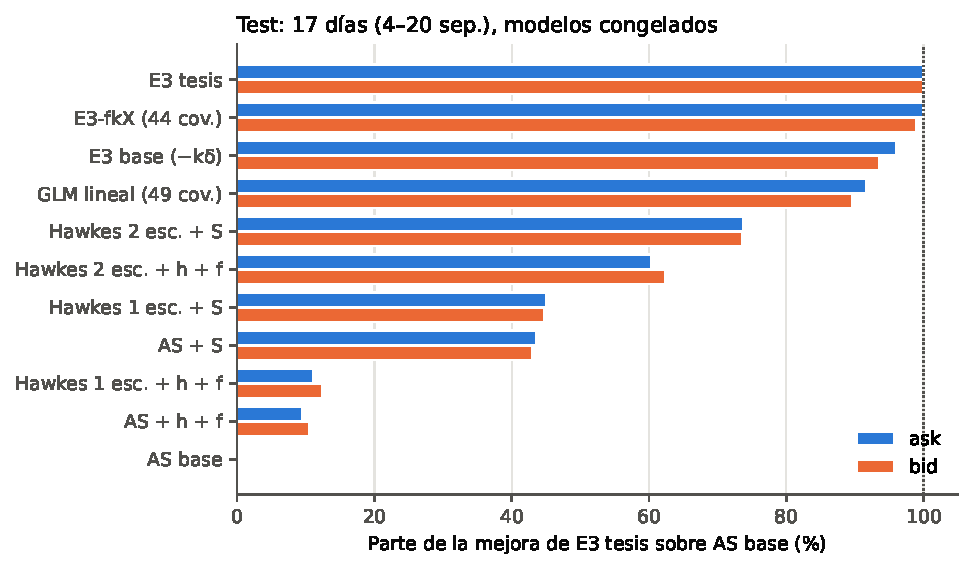
\includegraphics[width=.86\textwidth]{F4_parte_mejora_test.pdf}
\caption{Parte de la mejora de E3 tesis sobre AS base que recupera cada modelo en el test final.}
\label{fig:test-parte}
\end{figure}


\section{P1: calibración tras barridos}
\label{sec:rebote}

La Figura~\ref{fig:rebote} muestra, para el \textit{walk-forward}, la brecha entre la razón O/E del lado contrario tras barridos y la razón O/E habitual, separada por el lado del barrido y por la tendencia de la última hora. Cero indica que el modelo acierta tras un barrido tan bien como en momentos normales.

\begin{figure}[htbp]
\centering
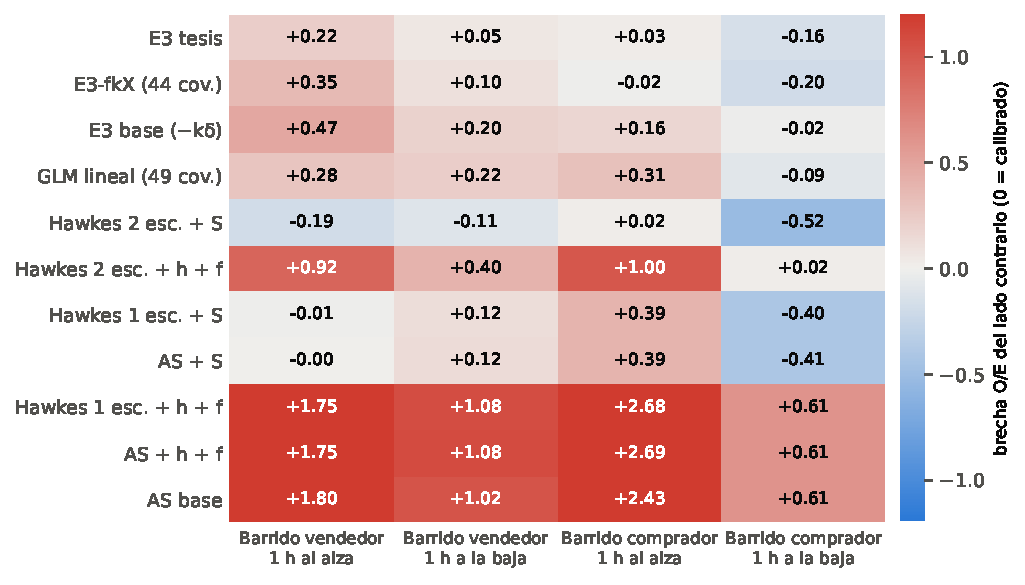
\includegraphics[width=.86\textwidth]{F3_rebote.pdf}
\caption{Brecha del rebote tras barridos en el \textit{walk-forward}, por modelo y situación. Rojo: llegan más agresores del lado contrario de los que el modelo espera; azul: menos.}
\label{fig:rebote}
\end{figure}

Los modelos sin covariables de estado (AS y Hawkes con h y f) subestiman fuertemente el rebote, con brechas de $+0{,}6$ a $+2{,}7$. Las señales lineales lo sobrecorrigen en la celda ``comprador con tendencia bajista'' ($-0{,}4$ a $-0{,}5$). E3 tesis tiene las brechas más cercanas a cero en tres de las cuatro celdas. La celda ``comprador con tendencia bajista'' ($-0{,}16$) no la corrige ningún modelo y queda como limitación declarada. En el test, la celda más débil de E3 tesis es ``comprador con tendencia alcista'' ($-0{,}235$).


\section{P3: política óptima con intensidades estimadas}
\label{sec:politica}

La HJB \eqref{eq:hjb-theta} se resolvió numéricamente con un esquema de Euler implícito linealizado, incondicionalmente estable porque la matriz del sistema es una M-matriz, seguido de un paso de Newton sobre el régimen ergódico. El Hamiltoniano se calcula con la curva de distancia de cada modelo interpolada: $\log\Lambda_i(\delta)$ es lineal a trozos entre los nueve nodos de $\delta$ y se extiende con la pendiente del primer y del último tramo; en cada tramo el máximo de $\Lambda_i(\delta)(1-e^{-\gamma(\delta-p)})/\gamma$ tiene forma cerrada, y $H_i$ es el máximo sobre los tramos, con $\delta$ restringida a $[-5;40]$~bps. Para aplicarla cada segundo se precalculan tablas en $(\ln\sigma^2/A_a,\ln A_b/A_a)$ y, para E3 tesis y E3-fkX, también en $(m_a,m_b)$, con rangos tomados de seis días de entrenamiento. Antes de usarla en el test se verificó en el entrenamiento que:
\begin{itemize}[nosep]
\item con forma exponencial reproduce la solución de la Sección~\ref{sec:hjb-teoria} (diferencia máxima $10^{-14}$), que a su vez reproduce la solución lineal de \citet{Gueant2017};
\item el máximo por tramos coincide con una búsqueda exhaustiva en una rejilla fina (error relativo máximo $2\times10^{-8}$);
\item las distancias son monótonas en el inventario;
\item las tablas reproducen la solución exacta con un error p99 de a lo sumo 0,027~bps en todo $|q|\le10$.
\end{itemize}
Ninguna pendiente de tramo resultó menor que 0,16~bps$^{-1}$ y ninguna distancia óptima tocó los bordes del intervalo. La aversión $\gamma=0{,}01$ se eligió en la fase de desarrollo. La Tabla~\ref{tab:hjb} muestra cómo cambia la política con cada intensidad.

\begin{table}[htbp]
\centering\small
\caption{Distancia óptima en el ask con inventario nulo (bps), mediana en el test; $\gamma=0{,}01$, ajuste corregido. La HJB usa la curva de distancia interpolada; GLFT, una exponencial local.}
\label{tab:hjb}
\begin{tabular}{@{}lcc@{}}\toprule
Intensidad & HJB & GLFT\\\midrule
AS base (forma exponencial) & 1,55 & 1,49\\
E3 base (forma exponencial) & 1,50 & 1,51\\
AS, Hawkes y GLM con curva $f(\delta)$ & 1,11--1,14 & 1,48--1,49\\
E3 tesis & 0,85 & 1,25\\\bottomrule
\end{tabular}
\end{table}

Tres resultados responden a P3. Primero, en GLFT la distancia base no depende del nivel $A$, de modo que las referencias apenas mueven las cotizaciones respecto de AS. Segundo, la forma de la curva sí importa en la solución numérica: con la curva interpolada, los modelos con $f(\delta)$ cotizan unos 0,4~bps más cerca que con una exponencial, y E3 tesis, cuya pendiente cerca del precio medio depende del estado, unos 0,7~bps más cerca. Frente a la versión que aproxima cada intensidad por una exponencial local, el precio cotizado cambia en el 86--99\,\% de las decisiones de esos modelos. Tercero, el cociente $A_b/A_a$ que predice E3 sesga la política hacia un lado incluso con inventario nulo. Los valores negativos de la distancia, que cruzarían el precio medio, se acotan al mejor precio para mantener la orden pasiva.

\section{Valor económico en el test}
\label{sec:p2}
La Tabla~\ref{tab:pnl} y la Figura~\ref{fig:pnl} muestran el desempeño en el test de las tres políticas con las intensidades de los modelos del ajuste corregido, todas con el mismo simulador, la misma orden de 0,01~BTC y el mismo límite de inventario. El precio medio de BTC en el test fue de unos 78\,000~USDT, de modo que cada orden vale unos 780~USDT.

\begin{table}[htbp]
\centering\footnotesize
\caption{PnL de market making en el test (17 días), bruto de comisiones; ajuste corregido. HJB con curva de distancia interpolada; GLFT con exponencial local. PnL por ejecución con IC95 por días.}
\label{tab:pnl}
\setlength{\tabcolsep}{3.5pt}
\resizebox{\textwidth}{!}{%
\begin{tabular}{@{}llrrcr@{}}\toprule
Política & Intensidad & Ejec./día & PnL/día (USDT) & PnL por ejec. (bps) & Días $>0$\\\midrule
\multirow{4}{*}{Miope} & E3 tesis & 4\,222 & $-443$ & $-1{,}34$ [$-1{,}48$; $-1{,}19$] & 0/17\\
 & AS, Hawkes, GLM con $f(\delta)$ & 3\,806 & $-385$ & $-1{,}29$ [$-1{,}45$; $-1{,}14$] & 0/17\\
 & AS base y E3 base ($\delta=2$) & 1\,173 & $-121$ & $-1{,}32$ [$-1{,}84$; $-0{,}78$] & 4/17\\
 & $\delta$ fijo 0,5~bps & 6\,872 & $-720$ & $-1{,}34$ [$-1{,}42$; $-1{,}24$] & 0/17\\\midrule
\multirow{6}{*}{HJB} & E3 tesis & 2\,451 & $-253$ & $-1{,}32$ [$-1{,}42$; $-1{,}20$] & 0/17\\
 & E3 base & 1\,677 & $-175$ & $-1{,}34$ [$-1{,}51$; $-1{,}15$] & 0/17\\
 & GLM lineal & 2\,549 & $-262$ & $-1{,}32$ [$-1{,}40$; $-1{,}22$] & 0/17\\
 & Hawkes 2 esc. + S & 3\,543 & $-355$ & $-1{,}28$ [$-1{,}35$; $-1{,}18$] & 0/17\\
 & AS + h + f & 3\,982 & $-398$ & $-1{,}28$ [$-1{,}35$; $-1{,}18$] & 0/17\\
 & AS base & 2\,218 & $-219$ & $-1{,}26$ [$-1{,}37$; $-1{,}14$] & 0/17\\\midrule
\multirow{3}{*}{GLFT} & E3 tesis & 3\,008 & $-289$ & $-1{,}23$ [$-1{,}32$; $-1{,}11$] & 0/17\\
 & Hawkes 2 esc. + S & 2\,321 & $-228$ & $-1{,}25$ [$-1{,}36$; $-1{,}12$] & 0/17\\
 & AS base & 2\,223 & $-218$ & $-1{,}25$ [$-1{,}35$; $-1{,}13$] & 0/17\\\bottomrule
\end{tabular}}
\end{table}

\begin{figure}[htbp]
\centering
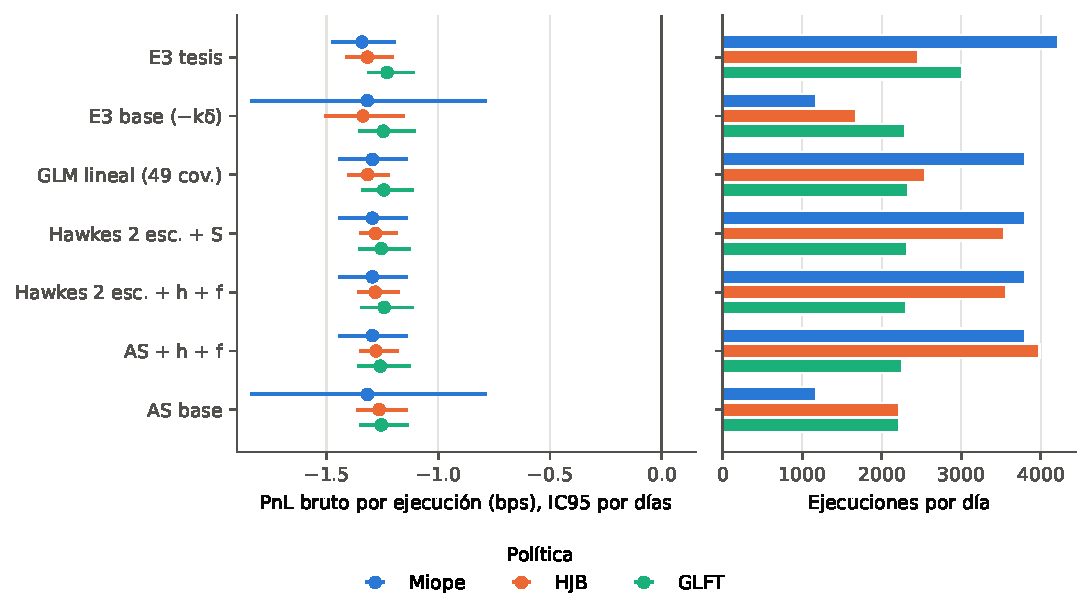
\includegraphics[width=.98\textwidth]{F5_pnl_test.pdf}
\caption{PnL bruto por ejecución (izquierda, IC95 por días) y ejecuciones por día (derecha) en el test, por intensidad y política; ajuste corregido, HJB con curva interpolada.}
\label{fig:pnl}
\end{figure}

\begin{itemize}[nosep]
\item \textbf{Las diferencias por ejecución entre combinaciones no son concluyentes.} Todas pierden entre $-1{,}22$ y $-1{,}34$~bps antes de comisiones, y las diferencias pareadas entre E3 tesis y cada referencia, en las tres políticas, tienen intervalos que incluyen el cero.
\item \textbf{E3 cambia la política, no el resultado por ejecución.} Con la HJB, E3 tesis opera entre un 31 y un 38\,\% menos que AS y Hawkes con la misma forma de curva (2\,451 frente a 3\,543--3\,982 ejecuciones por día) y pierde menos por día ($-253$ frente a $-355$ a $-398$~USDT); frente a AS base, con forma exponencial, opera un 10\,\% más. La pérdida por ejecución es similar en todos los casos.
\item \textbf{La curva interpolada cambia las cotizaciones, no la pérdida por ejecución.} Frente a la HJB con exponencial local, aumenta las ejecuciones entre 723 y 1\,735 por día según el modelo, con diferencias en el PnL por ejecución de $-0{,}04$ a $+0{,}02$~bps, todas con intervalos que incluyen el cero.
\item \textbf{La regla miope colapsa a distancias fijas.} Como solo usa la forma de $\lambda$ en $\delta$, los modelos con curva $f(\delta)$ fija eligen siempre 1~bps y los de forma exponencial siempre 2~bps; solo E3 tesis varía la distancia con el estado.
\item \textbf{Las comisiones agravan el resultado.} Con la comisión maker estándar de un participante minorista (7,5--10~bps por ejecución), todas las combinaciones pierden entre 9 y 11~bps por ejecución.
\end{itemize}

\section{Simulación del 21 de septiembre al 26 de octubre}
\label{sec:simulacion}

Con los mismos modelos y políticas, sin ningún reajuste, se evaluaron los 36 días posteriores al test. Antes de abrir el periodo se comprobó que el código reproduce exactamente un día del test (diferencia nula en predicción, ejecuciones y PnL).

\begin{table}[htbp]
\centering\footnotesize
\caption{Simulación (21 sep.--26 oct., 36 días; modelos congelados). Parte de la mejora sobre AS base, ventaja de E3 tesis por segundo [IC95 por días], días ganados y AUC (ask / bid).}
\label{tab:sim}
\resizebox{\textwidth}{!}{%
\begin{tabular}{@{}lrrcccc@{}}\toprule
& \multicolumn{2}{c}{Parte de la mejora} & \multicolumn{2}{c}{E3 tesis $-$ modelo} & & \\
\cmidrule(lr){2-3}\cmidrule(lr){4-5}
Modelo & ask & bid & ask & bid & Días & AUC\\\midrule
\textbf{E3 tesis} & 100\,\% & 100\,\% & -- & -- & -- & 0,848 / 0,842\\
E3-fkX (44 cov.) & 100,2\,\% & 99,3\,\% & $-0{,}003$ [$-0{,}010$; 0,005] & $+0{,}008$ [0,003; 0,014] & 16 / 28 & 0,848 / 0,842\\
E3 base & 94,5\,\% & 94,2\,\% & $+0{,}065$ [0,047; 0,085] & $+0{,}074$ [0,058; 0,092] & 33 / 36 & 0,847 / 0,842\\
GLM lineal (49 cov.) & 90,8\,\% & 90,0\,\% & $+0{,}107$ [0,071; 0,146] & $+0{,}129$ [0,077; 0,177] & 32 / 35 & 0,840 / 0,836\\
Hawkes 2 esc. + S & 70,2\,\% & 70,7\,\% & $+0{,}347$ [0,295; 0,406] & $+0{,}376$ [0,321; 0,441] & 36 / 36 & 0,785 / 0,783\\
Hawkes 2 esc. + h + f & 58,8\,\% & 62,2\,\% & $+0{,}479$ [0,389; 0,584] & $+0{,}486$ [0,403; 0,582] & 36 / 36 & 0,764 / 0,765\\
Hawkes 1 esc. + S & 43,6\,\% & 41,9\,\% & $+0{,}657$ [0,551; 0,770] & $+0{,}747$ [0,613; 0,892] & 36 / 36 & 0,746 / 0,743\\
AS + S & 41,9\,\% & 39,9\,\% & $+0{,}676$ [0,565; 0,795] & $+0{,}773$ [0,631; 0,927] & 36 / 36 & 0,743 / 0,740\\
Hawkes 1 esc. + h + f & 15,9\,\% & 16,1\,\% & $+0{,}979$ [0,793; 1,205] & $+1{,}079$ [0,852; 1,321] & 36 / 36 & 0,654 / 0,654\\
AS + h + f & 14,1\,\% & 13,9\,\% & $+0{,}999$ [0,809; 1,230] & $+1{,}107$ [0,873; 1,360] & 36 / 36 & 0,642 / 0,642\\
AS base & 0\,\% & 0\,\% & $+1{,}164$ [0,946; 1,419] & $+1{,}286$ [1,016; 1,575] & 36 / 36 & 0,500 / 0,500\\\bottomrule
\end{tabular}}
\end{table}

\paragraph{Predicción.} El orden de los modelos se mantiene y el AUC de E3 tesis sube a 0,85, sin degradación semana a semana (0,81 a 0,87 en las cinco semanas; 0,83 a 0,87 en las tres semanas desde el 5 de octubre). E3 tesis supera a todas las referencias con intervalos que excluyen el cero, salvo a E3-fkX en el lado ask, como en el test. De los cuatro criterios del test, escalados a 36 días, se cumplen los tres primeros (jerarquía, consistencia y AUC). El de calibración tras barridos no se cumple: la brecha es $+0{,}11$ tras barridos vendedores y $+0{,}22$ tras compradores, frente al límite de $\pm0{,}15$.

\paragraph{Valor económico.} Los resultados repiten los del test (Tabla~\ref{tab:sim-pnl}). Ninguna combinación de modelo y política es rentable. Con la HJB, las diferencias por ejecución entre E3 tesis y las referencias no son significativas. Con la regla miope, E3 tesis pierde $0{,}08$~bps más por ejecución que los modelos que cotizan siempre a 1~bps (IC95 $[-0{,}128; -0{,}028]$), porque se acerca al precio medio en los momentos de mayor intensidad predicha. Las tablas de la HJB cubren el periodo: en promedio, el 0,3--0,5\,\% de los segundos cae fuera de sus rangos.

\begin{table}[htbp]
\centering\footnotesize
\caption{PnL en la simulación (36 días), bruto de comisiones; modelos congelados, HJB con curva interpolada. PnL por ejecución con IC95 por días.}
\label{tab:sim-pnl}
\resizebox{\textwidth}{!}{%
\begin{tabular}{@{}llrrcr@{}}\toprule
Política & Intensidad & Ejec./día & PnL/día (USDT) & PnL por ejec. (bps) & Días $>0$\\\midrule
\multirow{3}{*}{Miope} & E3 tesis & 4\,406 & $-449$ & $-1{,}22$ [$-1{,}31$; $-1{,}14$] & 0/36\\
 & AS, Hawkes, GLM con $f(\delta)$ & 3\,869 & $-369$ & $-1{,}14$ [$-1{,}22$; $-1{,}07$] & 0/36\\
 & AS base ($\delta=2$) & 975 & $-98$ & $-1{,}20$ [$-1{,}52$; $-0{,}89$] & 9/36\\\midrule
\multirow{4}{*}{HJB} & E3 tesis & 2\,375 & $-249$ & $-1{,}26$ [$-1{,}34$; $-1{,}18$] & 0/36\\
 & GLM lineal & 2\,398 & $-250$ & $-1{,}25$ [$-1{,}32$; $-1{,}18$] & 0/36\\
 & Hawkes 2 esc. + S & 3\,612 & $-369$ & $-1{,}23$ [$-1{,}28$; $-1{,}18$] & 0/36\\
 & AS base & 2\,115 & $-212$ & $-1{,}20$ [$-1{,}27$; $-1{,}13$] & 1/36\\\midrule
\multirow{2}{*}{GLFT} & E3 tesis & 3\,065 & $-309$ & $-1{,}21$ [$-1{,}27$; $-1{,}15$] & 0/36\\
 & AS base & 2\,120 & $-213$ & $-1{,}20$ [$-1{,}27$; $-1{,}13$] & 1/36\\\bottomrule
\end{tabular}}
\end{table}

\section{Origen de la pérdida}
\label{sec:p2-origen}

Cada ejecución puede descomponerse en dos partes: la distancia capturada respecto del precio medio en el momento de la decisión y el movimiento posterior del precio medio. Su suma es el \textit{markout} \eqref{eq:markout}. La Tabla~\ref{tab:sa} la presenta para las ejecuciones del test y de la simulación.

\begin{table}[htbp]
\centering\footnotesize
\caption{Descomposición de la pérdida por ejecución (bps; media por ejecución): distancia capturada, movimiento posterior del precio medio y \textit{markout} a 10~s. Modelos congelados.}
\label{tab:sa}
\resizebox{\textwidth}{!}{%
\begin{tabular}{@{}llrrrrr@{}}\toprule
Periodo & Combinación & Capturada & Mov. 1~s & Mov. 10~s & \textit{Markout} 10~s & \% $>0$\\\midrule
\multirow{5}{*}{Test} & E3 tesis, miope & $+0{,}92$ & $-1{,}78$ & $-2{,}15$ & $-1{,}24$ & 23\\
 & E3 tesis, HJB & $+1{,}08$ & $-2{,}08$ & $-2{,}36$ & $-1{,}28$ & 27\\
 & Hawkes 2 esc. + S, HJB & $+1{,}01$ & $-1{,}96$ & $-2{,}28$ & $-1{,}27$ & 26\\
 & AS base, HJB & $+1{,}46$ & $-2{,}43$ & $-2{,}75$ & $-1{,}29$ & 29\\
 & AS base, miope ($\delta=2$) & $+2{,}00$ & $-3{,}04$ & $-3{,}31$ & $-1{,}31$ & 32\\\midrule
\multirow{3}{*}{Simulación} & E3 tesis, HJB & $+1{,}04$ & $-1{,}93$ & $-2{,}28$ & $-1{,}24$ & 27\\
 & AS base, HJB & $+1{,}46$ & $-2{,}30$ & $-2{,}64$ & $-1{,}18$ & 29\\
 & AS base, miope ($\delta=2$) & $+2{,}00$ & $-2{,}92$ & $-3{,}21$ & $-1{,}21$ & 32\\\bottomrule
\end{tabular}}
\end{table}

En los dos periodos y en todas las combinaciones se repite la misma regularidad. Lo que se captura de más al cotizar más lejos (de $+0{,}9$ a $+2{,}0$~bps) se pierde en un movimiento posterior mayor (de $-2{,}1$ a $-3{,}3$~bps), y el \textit{markout} queda entre $-1{,}16$ y $-1{,}31$~bps. Una cotización alejada solo se ejecuta cuando un barrido grande la atraviesa, y tras ese barrido el precio sigue en la misma dirección. Entre el 80 y el 90\,\% del movimiento a 10~s ocurre en el primer segundo, y solo entre el 23 y el 32\,\% de las ejecuciones resulta ganador. En BTC/USDT el spread es de un tick el 99,96\,\% del tiempo, así que el margen por cotizar procede únicamente de la distancia elegida, y esa distancia queda compensada por el movimiento posterior.

La pérdida tampoco depende de la intensidad que predice el modelo. Ordenando las ejecuciones de E3 tesis con la HJB por su intensidad predicha a 2~bps, la distancia capturada sube del decil más bajo al más alto (de 0,4 a 2,2~bps en el test), pero el \textit{markout} se mantiene entre $-1{,}0$ y $-1{,}4$~bps en el test y entre $-1{,}15$ y $-1{,}30$~bps en la simulación. Con la regla miope, el decil de mayor intensidad es el que más pierde ($-1{,}39$~bps en el test y $-1{,}25$~bps en la simulación).

En las configuraciones probadas en el entrenamiento, el resultado fue robusto al simulador, al modelo de cola y a la latencia. La regla de ejecución usada aquí coincide con simuladores que modelan la cola explícitamente: con hftbacktest, a 0,01--0,06~bps por ejecución; con NautilusTrader, entre $-1{,}22$ y $-1{,}27$~bps frente a $-1{,}26$. Reducir la latencia simulada de 100~ms a 10~$\mu$s deja la pérdida entre $-1{,}21$ y $-1{,}28$~bps. Estas comprobaciones, con políticas simétricas cerca del mejor precio, no cubren el test ni otras políticas, y los datos de 100~ms no permiten simular cancelaciones en microsegundos. Otras pruebas exploratorias de la parte económica, ninguna rentable después de comisiones, se resumen en el Apéndice~\ref{app:p2-exploratorio}.

\section{Avance frente a los objetivos}

\begin{table}[htbp]
\centering\small
\caption{Cumplimiento de los objetivos específicos.}
\label{tab:avance-oe}
\begin{tabular}{@{}p{.07\textwidth}p{.84\textwidth}@{}}\toprule
OE & Evidencia\\\midrule
OE1 & E1 estimado por lado; su forma exponencial queda mal calibrada por distancia y su nivel constante deja el AUC en 0,5. En la política, la distancia base depende de $k$ y no de $A$ (Secciones~\ref{sec:especificacion-final} y~\ref{sec:politica}).\\
OE2 & Intensidad \eqref{eq:fkx} con 49 covariables, $h$ horaria, curva monótona y modulación por estado; ablaciones y calibración tras barridos (Sección~\ref{sec:especificacion-final}).\\
OE3 & GBM y \textit{Random Forest} comparados con la misma información: conclusiones iguales, GBM más eficiente (Sección~\ref{sec:especificacion-final}).\\
OE4 & HJB derivada y resuelta numéricamente con intensidades dependientes del estado, verificada contra soluciones conocidas y aplicada en el test (Sección~\ref{sec:politica}).\\
OE5 & Comparación económica en el test frente a AS y Hawkes, con PnL, inventario y selección adversa; robustez entre ventanas, simuladores, colas y latencias (Secciones~\ref{sec:walkforward} y~\ref{sec:p2}).\\\bottomrule
\end{tabular}
\end{table}
\chapter{Discusión}
\label{chap:discusion}

\section{Qué aporta la estimación semiparamétrica}

La evidencia predictiva favorece a E3 frente a las referencias principales. La ventaja aparece en las cinco ventanas del \textit{walk-forward} y se mantiene en el test y en el periodo posterior. Sin embargo, la comparación con referencias reforzadas acota su magnitud: en el test, el mejor Hawkes recupera cerca del 74\,\% de la mejora sobre AS y el modelo lineal con las mismas covariables, alrededor del 90\,\%. El estado del mercado aporta, por tanto, la mayor parte de la información que falta a la intensidad constante.

La ventaja restante corresponde a la especificación flexible de E3, incluida su modulación de la curva. No puede atribuirse íntegramente a la no linealidad de $g$ mediante la comparación con el GLM, porque las especificaciones difieren también en otros componentes. Las ablaciones muestran además que las variables de barrido aportan poco a la puntuación global, pero ayudan a corregir el nivel de las predicciones tras esos eventos. Frente a E3-fkX, esa aportación global no es significativa en el ask del test ni de la simulación. La calibración sigue siendo una limitación: el criterio tras barridos compradores falla en el periodo posterior.

Estas conclusiones responden a P1 y a la estabilidad temporal de P4. Se refieren al número esperado de eventos que alcanzan una distancia. Un AUC alto en esa tarea no mide acierto en la dirección del precio, probabilidad de beneficio ni ejecución de una orden propia.

\section{De la intensidad a la política y al resultado económico}

La intensidad estimada sí modifica la política, lo que responde a P3. La curva de distancia y la asimetría entre lados cambian las cotizaciones HJB con coeficientes congelados. En el test, con cruce estricto, E3 tesis ejecuta entre un 31 y un 38\,\% menos que AS y Hawkes con la misma forma de curva, y pierde menos por día. Esta reducción no equivale a una ventaja por ejecución: las diferencias pareadas de PnL por nocional no son significativas en ese periodo.

La respuesta a P2 depende de la regla de ejecución. Bajo cruce estricto y FIFO aproximada, el PnL bruto agregado es negativo. Bajo toque optimista, la HJB con E3 obtiene ganancias brutas pequeñas y supera a AS y Hawkes; E3 base, que no es la mejor especificación predictiva, presenta el mejor resultado económico entre las variantes de E3. Ninguno cubre las comisiones evaluadas. Por tanto, no se establece una correspondencia entre el orden predictivo de las intensidades y el orden económico de las políticas.

\section{Cómo interpretar las pérdidas}

La pérdida bajo cruce estricto no se explica solo por las comisiones: aparece antes de aplicarlas. La descomposición de la Sección~\ref{sec:p2-origen} muestra que la captura respecto del mid de decisión es positiva, pero el movimiento asociado a las ejecuciones es mayor y de signo contrario. Cotizar más lejos aumenta el margen inicial y reduce las ejecuciones; no garantiza mejor calidad en las que sí ocurren. Esta regularidad es compatible con selección adversa bajo la regla evaluada.

La interpretación concuerda con \citet{GlostenMilgrom1985}, para quienes el spread compensa el riesgo de negociar con agentes mejor informados, y con la evidencia empírica reciente en microestructura de alta frecuencia: la disyuntiva entre probabilidad de ejecución y retorno posterior documentada por \citet{AlbersEtAl2025} en futuros de Bitcoin en Binance, la deriva condicional negativa tras la ejecución de una orden límite estudiada por \citet{DeLise2024}, y el deterioro de la estrategia de control estocástico que \citet{LalorSwishchuk2024} examinan al introducir ejecuciones adversas y probabilidades de fill no adverso más realistas. La precisión estadística y el valor económico responden, por tanto, a criterios distintos \citep{LeitchTanner1991}.

Conviene separar selección adversa y gestión del inventario \citep{Menkveld2013}. El markout describe el valor de cada ejecución a un horizonte fijo; el PnL diario incorpora toda la trayectoria de las posiciones. Su semejanza de signo no identifica qué parte exacta del PnL causa cada mecanismo. La evidencia presentada respalda un deterioro alrededor de las ejecuciones y una menor pérdida total al operar menos; no demuestra que ajustar únicamente la aversión al inventario elimine ese deterioro.

La persistencia de resultados similares en los dos periodos refuerza la descripción bajo cruce estricto, pero no constituye una ley del mercado. Los eventos están agrupados, los modelos comparten reglas y parte de los datos había sido consultada. La excepción de R1 es decisiva: el conjunto de ejecuciones admitidas puede cambiar el signo bruto. Por ello, no se concluye que toda provisión de liquidez en BTC/USDT sea necesariamente deficitaria ni que la prioridad real sea irrelevante.

La comparación con motores alternativos sirve como comprobación auxiliar en configuraciones de entrenamiento. No valida de forma conjunta las políticas finales, la latencia real, las cancelaciones ni la posición en la cola de una orden en producción. La contribución económica es delimitar lo que no se monetizó bajo estos supuestos, sin convertir una explicación descriptiva en una afirmación causal universal.

\section{Limitaciones}
\label{sec:limitaciones}

\paragraph{Independencia de la evaluación.}
El test del 4 al 20 de septiembre no es completamente ciego: la especificación original de E3 ya se había evaluado allí, y una política de pausa se ejecutó antes de una orden de espera, aunque sus resultados no se consultaron. Las especificaciones finales se congelaron antes de su evaluación, pero esto no recupera la independencia del periodo. El \textit{walk-forward} se realizó dentro del bloque de desarrollo; sus ajustes respetan el orden temporal, sin constituir una selección anidada e independiente de toda la especificación.

La primera parte del periodo posterior, del 21 de septiembre al 6 de octubre, se usó en evaluaciones predictivas y económicas de versiones anteriores. Sus resultados no se usaron para seleccionar ni ajustar las especificaciones finales, pero ese tramo no es ciego en sentido estricto. Del 7 al 26 de octubre solo se construyó y verificó la capa de datos; ningún modelo se evaluó allí antes de la simulación.

\paragraph{Estimación y versiones del ajuste.}
Los Hawkes se estimaron con un tercio de los días por costo computacional, aunque sus capas de nivel, forma y señales usan todos. E3 utiliza tres ciclos de \textit{backfitting}, sin demostrar convergencia conjunta. En la versión original no se comprobaba la convergencia del último ajuste de la curva y el gradiente de $m(X)$ omitía el recorte de $b^\top z$ a $\pm5$, activado en unos 30 de 5,8 millones de segundos. La corrección verificó la convergencia de ese paso con $g$ y $h$ fijos. La curva cambia principalmente a 15--20~bps y el test conserva, a tres decimales, las ventajas de log-verosimilitud y el AUC. El \textit{walk-forward} conserva el ajuste original. Esta comprobación no cuantifica todo el efecto de una eventual convergencia conjunta incompleta.

\paragraph{Alcance, ejecución y prioridad.}
La respuesta estadística mide alcance, no fills propios. Mejorar su predicción no implica mejorar la predicción de las ejecuciones que obtendría un agente. R2 usa profundidad visible o imputada, no cuenta cancelaciones delante de la orden y pierde la prioridad al recotizar; R1 supone ejecución completa al toque sin cola delante. Son escenarios de sensibilidad, no cotas demostradas del PnL real. La resolución de 100~ms y los veinte niveles no permiten reconstruir la prioridad efectiva. La sensibilidad de la HJB con E3 impide generalizar su resultado bruto a cualquier regla de cola.

\paragraph{Control y condiciones de operación.}
La HJB usa coeficientes congelados, una curva interpolada en nueve nodos y tablas numéricas; no incorpora la dinámica de $X_t$ como estado. GLFT añade una aproximación exponencial local. La evaluación final supone activación al inicio del segundo sin latencia de envío, no los aproximadamente 130~ms de red observados en la captura. El inventario terminal se marca al mid, sin liquidación ejecutada, impacto propio ni costo de salida. Las sensibilidades anteriores de motores y latencia no cubren todas las políticas finales ni carreras de cancelación en microsegundos \citep{BudishCramtonShim2015,AquilinaBudishONeill2022}.

\paragraph{Incertidumbre y generalización.}
Los conteos están anidados por distancia y la puntuación Poisson es compuesta; evalúa la media, no la distribución conjunta. El remuestreo por días recoge la dependencia intradía, pero no garantiza independencia entre días. La calibración tras barridos sigue siendo inestable. El estudio se refiere a un mercado y a unas comisiones concretas: no demuestra ausencia de valor en otros activos, tarifas, plataformas o mecanismos de ejecución.

% ═══════════════════════════════════════════════════════════════════════════
\chapter{Conclusiones y trabajo futuro}
\label{chap:conclusiones}
% ═══════════════════════════════════════════════════════════════════════════

Este trabajo propuso y evaluó una intensidad semiparamétrica de llegada de órdenes agresivas para market making en BTC/USDT, $\lambda_i(t,\delta\mid X_t)=\exp\{g_i(X_t)+h_i(t)+m_i(X_t)f_i(\delta)\}$, y la comparó con Avellaneda--Stoikov y con un Hawkes bivariado reforzados con los mismos hallazgos. Las conclusiones son:

\begin{enumerate}
\item \textbf{La intensidad semiparamétrica predice mejor.} Supera a las referencias en las cinco ventanas del \textit{walk-forward}, en el test y en una simulación posterior de 36 días sin reajustes, en ambos lados del libro, con un AUC de 0,81--0,85. Los intervalos de confianza por días excluyen el cero frente a todas las referencias, salvo frente a E3-fkX en el lado ask, donde la diferencia no es significativa en el test ni en la simulación. Se cumplieron todos los criterios preregistrados del \textit{walk-forward} y del test; en la simulación falló el de calibración tras barridos.
\item \textbf{La ganancia proviene sobre todo del estado del mercado.} Un modelo lineal con las mismas covariables recupera el 90\,\%; la no linealidad añade el resto y, frente a las referencias evaluadas, mejoró la discriminación y la calibración tras barridos. El Hawkes recupera el 60--74\,\% solo cuando tiene dos escalas de memoria.
\item \textbf{La forma en la distancia importa.} Una curva monótona modulada por el estado corrige la mala calibración de $e^{-k\delta}$, y las covariables de barrido corrigen la subestimación del rebote en tres de cuatro situaciones.
\item \textbf{La estimación \textit{data-driven} cambia la política de cotización.} La HJB resuelta numéricamente y aplicada con coeficientes congelados, con la curva de distancia interpolada, se sesga según el cociente de intensidades entre lados y según la pendiente de la curva; con E3 opera entre un 31 y un 38\,\% menos que AS y Hawkes con la misma forma de curva. En la aproximación cerrada GLFT, el nivel de la intensidad solo entra en el término de inventario, porque la distancia base $\gamma^{-1}\log(1+\gamma/k_i)$ no depende de $A_i$.
\item \textbf{Ninguna política es rentable neta de las comisiones evaluadas.} Con la regla de cruce estricto, con cualquier intensidad y cualquiera de las tres políticas, el market making pasivo pierde aproximadamente entre 1,1 y 1,3~bps por ejecución antes de comisiones, en el test y en la simulación; con una cola FIFO aproximada el resultado no cambia. La excepción es la HJB con E3 bajo una ejecución optimista al toque, sin cola delante: obtiene una ganancia bruta pequeña en la simulación (de $+0{,}15$~bps por ejecución con E3 tesis a $+0{,}44$~bps con E3 base) y supera a AS y Hawkes, pero no cubre las comisiones de 7,5--10~bps. Bajo cruce estricto, lo que se captura al cotizar más lejos queda compensado por un movimiento posterior mayor del precio, la mayor parte en el primer segundo: es selección adversa en un mercado con spread de un tick. Con cruce estricto, las diferencias entre modelos son pequeñas; la única significativa es que, con la regla miope, E3 pierde 0,08~bps más por ejecución en la simulación.
\end{enumerate}

La contribución del trabajo es, por tanto, predictiva, y su resultado económico es negativo neto de las comisiones evaluadas. Ambos se sustentan con el mismo protocolo: datos propios auditados, especificaciones congeladas antes de evaluar y criterios fijados de antemano. El periodo de test había sido consultado antes con una versión anterior del modelo, y congelar una versión nueva no recupera su independencia.

\paragraph{Trabajo futuro.}
\begin{itemize}[nosep]
\item Modelar conjuntamente la probabilidad de ejecución y el \textit{markout} posterior, que es la cantidad económicamente relevante. En la fase exploratoria, las covariables disponibles explicaron menos del 3\,\% de la variación del \textit{markout} por ejecución, por lo que su valor con datos de 100~ms es dudoso.
\item Repetir la comparación en mercados con spread más ancho o con comisión maker nula o negativa, y en otras plataformas como Coinbase BTC-USD, donde la ventaja predictiva podría monetizarse.
\item Incorporar $X_t$ como variable de estado en la HJB, en lugar de coeficientes congelados.
\item Medir la prioridad real en la cola con datos del libro por mensaje, y estimar el resultado de la HJB con E3 sin depender de los escenarios de cola de este trabajo.
\item Medir la latencia propia en operación real o capturar desde la región del motor de Binance, para estudiar las carreras de cancelación que los datos de 100~ms no permiten simular.
\end{itemize}


\appendix
% ═══════════════════════════════════════════════════════════════════════════
\chapter{Covariables y disponibilidad del código}
\label{app:trazabilidad}
% ═══════════════════════════════════════════════════════════════════════════

\section{Covariables de E3}
Las 49 covariables se calculan con información disponible antes de cada decisión (Tabla~\ref{tab:covariables}). Las ventanas \texttt{past\_*} excluyen el intervalo actual. Las covariables de barrido usan transacciones estrictamente anteriores y superan la prueba automática de truncamiento.

\begin{table}[htbp]
\centering\footnotesize
\caption[Covariables de E3 por grupo.]{Covariables de $g(X_t)$ por grupo.}
\label{tab:covariables}
\begin{tabular}{@{}p{.15\textwidth}rp{.68\textwidth}@{}}\toprule
Grupo & $n$ & Variables\\\midrule
Libro & 15 & spread; desequilibrio en los niveles 1, 5 y 20 y ponderado; prima del microprecio; profundidad de compra y venta en 5 y 20 niveles; pendiente del libro por lado; entropía de la profundidad por lado; antigüedad del libro\\
OFI & 4 & OFI ponderado en 1, 5 y 20 niveles; OFI de 5 niveles\\
Volatilidad & 5 & volatilidad realizada a 1, 5, 10 y 60~s; variación del precio medio en 100~ms\\
Flujo & 20 & número y volumen de compras y ventas agresoras, y volumen firmado, en ventanas de 1, 5, 30 y 60~s\\
Barridos & 5 & recorrido firmado, volumen y tiempo desde el último barrido (evento agresor que recorre al menos 0,5~bps, en los últimos 60~s); spread máximo del último segundo; variación del precio medio en el último segundo\\\bottomrule
\end{tabular}
\end{table}

La modulación $m(X)$ usa cuatro covariables estandarizadas: volatilidad realizada a 10~s, $\log(1+\text{transacciones en 5~s})$, logaritmo de la profundidad propia en cinco niveles y desequilibrio en cinco niveles. Las siete señales S de las referencias son las cinco de barrido y las variaciones del precio medio en 15~min y 1~h.

\section{Disponibilidad y verificación}
El código, los protocolos de cada etapa y los modelos finales están en el repositorio del proyecto:
\begin{center}\url{https://github.com/sannti09/market-making-semiparametrico}\end{center}
 La versión del código que corresponde a este documento es el \textit{commit} \texttt{69af855}. Esta revisión editorial V3 actualiza la exposición y conserva los modelos y resultados publicados; las correcciones de código refuerzan su reproducción. El repositorio es público: el código se distribuye con licencia MIT y este documento con licencia Creative Commons Atribución 4.0 (CC BY 4.0). Cada protocolo se escribió y fechó antes de correr la etapa correspondiente, y el código comprueba al ejecutarse que el protocolo no cambió. Los modelos finales se guardaron antes de leer el test. El repositorio incluye además el catálogo de los archivos de datos, que permite verificar que cualquier réplica usa exactamente los mismos datos.

\chapter{Desarrollo y evaluación de la especificación original}
\label{app:ciegos}

\section{Fase de desarrollo}
La Tabla~\ref{tab:intensidades} compara la especificación original de E3 con AS y con el Hawkes de una escala en la calibración interna (13--16 de julio), con hiperparámetros elegidos en ese mismo bloque.

\begin{table}[htbp]
\centering\small
\caption[Comparación en la fase de desarrollo.]{Fase de desarrollo. Log-verosimilitud en calibración interna (4 días, 345\,600 intervalos por lado) y AUC medio ($\delta=2$~bps). Mayor es mejor.}
\label{tab:intensidades}
\begin{tabular}{@{}lrrrr@{}}\toprule
Modelo & $\ell$ ask & $\ell$ bid & AUC ask & AUC bid\\\midrule
E1: $Ae^{-k\delta}$ & $-903\,215$ & $-803\,621$ & 0,500 & 0,500\\
E1 $+h$(hora) & $-789\,821$ & $-758\,297$ & 0,695 & 0,676\\
E2: Hawkes de una escala & $-886\,725$ & $-794\,714$ & 0,643 & 0,653\\
\textbf{E3: GBM} & $\mathbf{-418\,255}$ & $\mathbf{-468\,377}$ & \textbf{0,840} & \textbf{0,843}\\
E3: \textit{Random Forest} & $-423\,078$ & $-467\,767$ & 0,840 & 0,844\\\bottomrule
\end{tabular}
\end{table}

\section{Validación y tests ciegos}

Antes de reforzar los modelos, la especificación original de E3 se evaluó en tres bloques que no se usaron para elegirla. La Tabla~\ref{tab:ciegos} resume los resultados.

\begin{table}[htbp]
\centering\small
\caption[Evaluación de la especificación original.]{E3 original frente a E1 en bloques posteriores al desarrollo: días en que gana E3, mejora por intervalo [IC95 por días] y AUC.}
\label{tab:ciegos}
\begin{tabular}{@{}lcccc@{}}\toprule
Bloque & Días & Mejora ask & Mejora bid & AUC ask / bid\\\midrule
Validación (17--23 jul.) & 7/7 & 0,85 [0,72; 1,03] & 0,92 [0,69; 1,26] & 0,806 / 0,802\\
Ciego 1 (26 ago.--15 sep.) & 21/21 & 1,30 [0,96; 1,69] & 1,29 [0,87; 1,79] & 0,810 / 0,798\\
Ciego 2 (16 sep.--6 oct.) & 21/21 & 1,13 [0,79; 1,51] & 1,39 [0,95; 1,88] & 0,831 / 0,828\\\bottomrule
\end{tabular}
\end{table}

E3 superó a E1 y a E1 con efecto horario en todos los días de los tres bloques y en ambos lados. Los veredictos preregistrados fueron: validación cumplida; ciego~1 no cumplido; ciego~2 cumplido. En el ciego~1 fallaron dos criterios. El AUC del lado bid quedó en 0,798, por debajo del umbral de 0,80. El cociente entre la mejora del bloque y la de referencia quedó en 0,23--0,25, porque la referencia elegida (18--21 de agosto) correspondía a días extremos; fue un error de diseño del protocolo, que se reporta sin cambios.

Un GLM lineal con las mismas 44 covariables recuperaba el 88--93\,\% de la mejora de E3, pero con un AUC de 0,78--0,79, por debajo del umbral; E3 le ganó en AUC todos los días.


\chapter{Pruebas exploratorias de la parte económica}
\label{app:p2-exploratorio}

Estas pruebas se hicieron en el entrenamiento, o en bloques ya vistos, para buscar una vía rentable o entender la pérdida. Ninguna fue rentable después de comisiones; algunas variantes agresivas tuvieron un resultado bruto positivo. Se resumen para que el lector conozca qué se intentó.

\paragraph{Por qué algunos \textit{backtests} intermedios parecieron mucho mejores.} Un simulador que daba por ejecutadas como pasivas cotizaciones que en realidad habrían cruzado el libro reducía artificialmente la pérdida de $-1{,}26$ a $-0{,}2$~bps por ejecución; la validación con cola explícita lo detectó y ese resultado se retiró. Otras métricas excluían las operaciones perdedoras (por ejemplo, contar solo ciclos cerrados con un precio mínimo de salida) o comparaban con mantener la posición, lo que mide la dirección del inventario y no la provisión de liquidez.

\paragraph{Pausa defensiva.} Retirar las cotizaciones cuando un modelo de saltos anticipa alta probabilidad de un movimiento brusco reduce la pérdida entre 0,03 y 0,09~bps por ejecución, con intervalos que excluyen el cero, pero la mejor combinación queda en $-1{,}03$~bps y ningún día es positivo. Saber \emph{cuándo} habrá un salto es posible (AUC 0,81--0,91); saber \emph{hacia dónde} acierta el 58--60\,\% de las veces, frente al 54\,\% que se obtiene prediciendo siempre la dirección más frecuente.

\paragraph{Spreads anchos.} Un spread de al menos 1~bps aparece en promedio 1,4~s al día. El 85--96\,\% de esos episodios los abre un barrido, tras el cual el precio sigue en la dirección del barrido. Incluso suponiendo una ejecución asegurada en esos instantes, el resultado a 10~s es de $-3{,}9$ a $-5{,}9$~bps.

\paragraph{Operar como agresor.} Una señal de dirección a 10~s construida con las covariables de E3 captura entre 0,65 y 0,8~bps por orden antes de comisiones; seguir la dirección de un barrido tras un spread ancho no supera de forma robusta el umbral de comisión. Ninguna variante probada cubre la comisión de ida y vuelta de un participante minorista.

\paragraph{Información externa.} En las pruebas realizadas, los perpetuos de otras plataformas mejoraron la predicción de dirección frente a un modelo lineal simple, pero no frente a un GBM con las covariables propias del libro; otras criptomonedas, índices bursátiles y opciones no mostraron una anticipación útil a los horizontes evaluados.


\backmatter
\bibliographystyle{plainnat}
\bibliography{references_final}
\end{document}
